%!TEX root = ../thesis.tex
% ************************** Thesis Abstract *****************************
% 4eme de couverture
\ifthispageodd{\newpage\thispagestyle{empty}\null\newpage}{}
\thispagestyle{empty}
\newgeometry{top=1.5cm, bottom=1.25cm, left=2cm, right=2cm}
%\fontfamily{rm}\selectfont

\lhead{}
\rhead{}
\rfoot{}
\cfoot{}
\lfoot{}

\noindent 
%*****************************************************
%***** LOGO DE L'ED À CHANGER ÉVENTUELLEMENT *********
%*****************************************************

\includegraphics[height=2.45cm]{Figs/EOBE.png}
\vspace{1cm}
%*****************************************************

\begin{mdframed}[linecolor=Prune,linewidth=1]
\vspace{-.25cm}
\paragraph*{Titre:} 
Analyse d'une nouvelle topologie fiable de convertisseur analogique-numérique pour \newline l'environnement automobile
% \begin{small}
\vspace{-.25cm}
\paragraph*{Mots clés:} 

\vspace{-.5cm}
\paragraph*{Résumé:} 
L'électronique automobile voit une forte expansion de la demande de capteurs intelligents avec une intégration de plus en plus poussée. Capteurs, interfaces, contrôleurs ayant la puissance de calcul se trouvent de plus en plus en un seul composant. De ce fait, les contraintes de stress mécanique et thermique deviennent des facteurs importants lors de la conception de convertisseur analogique-numérique ou de convertisseur numérique-analogique.

Dans le cadre de cette thèse, nous nous focalisons sur la conception d'un convertisseur analogique-numérique servant pour la conversion de signaux issus de capteurs de température, pression, courant, mais aussi pour une future application, en tant que convertisseur dans une chaîne de conversion de télécommunication. Le challenge de la conception d'un tel ADC réside dans la forte contrainte de rapidité et de résolution sur une plage de températures importantes: de -40 $\degree$C à +175 $\degree$C.

Ayant une contrainte économique d’autant plus importante, le cout réduit sera issu de la faible surface de silicium de ce composant alliée à une économie mondialisée que le secteur automobile connaît. Comme exposé dans le tableau~\ref{tbl:adc-spec-fr}, la surface n’excédera pas 0.5 $\rm mm^2$. Il est toutefois important de noter que le ratio entre la fréquence d'horloge maximale et la fréquence d'échantillonnage est seulement de 5. Ce ratio lié au sur-échantillonnage est très faible pour réaliser une conversion de 12 bits de résolution.

\begin{center}
    \centering
    \caption[]{Spécification du convertisseur analogique-numérique}
    \label{tbl:adc-spec-fr}
    \rowcolors{2}{gray!15}{white}
    \begin{tabular}{ll}
        \toprule
                                     & Critères                                                                                                                                                   \\ \midrule
    Plage de Température            & -40 $\degree$ C -- +175 $\degree$ C                                                                                               \\
    Tension d'alimentation                   & 1.8 V $\pm$ 10 \%                                                                                                                              \\
    Plage de la tension différentielle d'entrée & $\pm$ 1V                                                                                                                                       \\
    Surface                             & \textless 0.5 \(mm^2\)                                                                                                                                      \\
    Fréquence d'échantillonnage       & 20 MSamples/s                                                                                                                                               \\
    Fréquence d'horloge maximum      & 100 MHz
    Duty-Cycle de l'horloge                & 40 -- 60 \%                                                                                                                                                 \\
    Latence                          & 500 ns                                                                                                                                                      \\
    Résolution                       & $\geq$ 12-bit                                                                                                                                     \\
    DNL                              & \textless LSB/2                                                                                                                                             \\
    INL                              & \textless LSB/2 best-fit                                                                                                                             \\
    Erreur d'Offset                     & \textless 4 LSB                                                                                                                                             \\
    Erreur de Gain                       & \textless 4 LSB                                                                                                                                             \\
    Erreur d'appariement entre deux ADCs      & \textless 4 LSB                                                                                                                                             \\
    Energie, $E_s = P/F_s$            & 0.75 nJ/échantillon      \\ \bottomrule                                                                                                                                       
    \end{tabular}
\end{center}

Suite à l’analyse architecturale de convertisseurs traditionnels et de leurs avancées dans le chapitre~\ref{sec:soa}, les avantages et les sources d’erreurs dans la partie analogique nous permettent de sélectionner les architectures pour la haute température. Pour en nommer quelques-uns, on retrouve dans l’état de l’art des convertisseurs du type \(\Sigma \Delta\), des SAR, et des convertisseurs Pipeline. Ceux-ci se trouvent être moins sensibles à la variation de performance de ou des amplificateurs éventuels, et permettent, avec une calibration en un seul point en température, de compenser ces imperfections.

La section~\ref{sec:temperature-analogue} discute des challenges que pose la conception analogique en haute et basse température. Les phénomènes physiques en jeu sont analysés en fonction de la température afin de déduire les compromis existant auxquels nous devrons faire face. Basé sur une méthodologie \(g_m/I_D\), le résultat cette analyse est directement exploitable pour la phase de conception analogique.

\begin{center}
    \centering
    %% Creator: Matplotlib, PGF backend
%%
%% To include the figure in your LaTeX document, write
%%   \input{<filename>.pgf}
%%
%% Make sure the required packages are loaded in your preamble
%%   \usepackage{pgf}
%%
%% Figures using additional raster images can only be included by \input if
%% they are in the same directory as the main LaTeX file. For loading figures
%% from other directories you can use the `import` package
%%   \usepackage{import}
%% and then include the figures with
%%   \import{<path to file>}{<filename>.pgf}
%%
%% Matplotlib used the following preamble
%%   \usepackage{gensymb}
%%   \usepackage[utf8x]{inputenc}
%%   \usepackage[T1]{fontenc}
%%
\begingroup%
\makeatletter%
\begin{pgfpicture}%
\pgfpathrectangle{\pgfpointorigin}{\pgfqpoint{5.999954in}{3.930000in}}%
\pgfusepath{use as bounding box, clip}%
\begin{pgfscope}%
\pgfsetbuttcap%
\pgfsetmiterjoin%
\definecolor{currentfill}{rgb}{1.000000,1.000000,1.000000}%
\pgfsetfillcolor{currentfill}%
\pgfsetlinewidth{0.000000pt}%
\definecolor{currentstroke}{rgb}{1.000000,1.000000,1.000000}%
\pgfsetstrokecolor{currentstroke}%
\pgfsetdash{}{0pt}%
\pgfpathmoveto{\pgfqpoint{0.000000in}{0.000000in}}%
\pgfpathlineto{\pgfqpoint{5.999954in}{0.000000in}}%
\pgfpathlineto{\pgfqpoint{5.999954in}{3.930000in}}%
\pgfpathlineto{\pgfqpoint{0.000000in}{3.930000in}}%
\pgfpathclose%
\pgfusepath{fill}%
\end{pgfscope}%
\begin{pgfscope}%
\pgfsetbuttcap%
\pgfsetmiterjoin%
\definecolor{currentfill}{rgb}{1.000000,1.000000,1.000000}%
\pgfsetfillcolor{currentfill}%
\pgfsetlinewidth{0.000000pt}%
\definecolor{currentstroke}{rgb}{0.000000,0.000000,0.000000}%
\pgfsetstrokecolor{currentstroke}%
\pgfsetstrokeopacity{0.000000}%
\pgfsetdash{}{0pt}%
\pgfpathmoveto{\pgfqpoint{0.363168in}{0.485823in}}%
\pgfpathlineto{\pgfqpoint{5.670702in}{0.485823in}}%
\pgfpathlineto{\pgfqpoint{5.670702in}{3.806667in}}%
\pgfpathlineto{\pgfqpoint{0.363168in}{3.806667in}}%
\pgfpathclose%
\pgfusepath{fill}%
\end{pgfscope}%
\begin{pgfscope}%
\pgfsetbuttcap%
\pgfsetroundjoin%
\definecolor{currentfill}{rgb}{0.000000,0.000000,0.000000}%
\pgfsetfillcolor{currentfill}%
\pgfsetlinewidth{0.803000pt}%
\definecolor{currentstroke}{rgb}{0.000000,0.000000,0.000000}%
\pgfsetstrokecolor{currentstroke}%
\pgfsetdash{}{0pt}%
\pgfsys@defobject{currentmarker}{\pgfqpoint{0.000000in}{-0.048611in}}{\pgfqpoint{0.000000in}{0.000000in}}{%
\pgfpathmoveto{\pgfqpoint{0.000000in}{0.000000in}}%
\pgfpathlineto{\pgfqpoint{0.000000in}{-0.048611in}}%
\pgfusepath{stroke,fill}%
}%
\begin{pgfscope}%
\pgfsys@transformshift{0.363168in}{0.485823in}%
\pgfsys@useobject{currentmarker}{}%
\end{pgfscope}%
\end{pgfscope}%
\begin{pgfscope}%
\pgftext[x=0.363168in,y=0.388600in,,top]{\fontsize{10.000000}{12.000000}\selectfont Faible}%
\end{pgfscope}%
\begin{pgfscope}%
\pgfsetbuttcap%
\pgfsetroundjoin%
\definecolor{currentfill}{rgb}{0.000000,0.000000,0.000000}%
\pgfsetfillcolor{currentfill}%
\pgfsetlinewidth{0.803000pt}%
\definecolor{currentstroke}{rgb}{0.000000,0.000000,0.000000}%
\pgfsetstrokecolor{currentstroke}%
\pgfsetdash{}{0pt}%
\pgfsys@defobject{currentmarker}{\pgfqpoint{0.000000in}{-0.048611in}}{\pgfqpoint{0.000000in}{0.000000in}}{%
\pgfpathmoveto{\pgfqpoint{0.000000in}{0.000000in}}%
\pgfpathlineto{\pgfqpoint{0.000000in}{-0.048611in}}%
\pgfusepath{stroke,fill}%
}%
\begin{pgfscope}%
\pgfsys@transformshift{3.016935in}{0.485823in}%
\pgfsys@useobject{currentmarker}{}%
\end{pgfscope}%
\end{pgfscope}%
\begin{pgfscope}%
\pgftext[x=3.016935in,y=0.388600in,,top]{\fontsize{10.000000}{12.000000}\selectfont Modéré}%
\end{pgfscope}%
\begin{pgfscope}%
\pgfsetbuttcap%
\pgfsetroundjoin%
\definecolor{currentfill}{rgb}{0.000000,0.000000,0.000000}%
\pgfsetfillcolor{currentfill}%
\pgfsetlinewidth{0.803000pt}%
\definecolor{currentstroke}{rgb}{0.000000,0.000000,0.000000}%
\pgfsetstrokecolor{currentstroke}%
\pgfsetdash{}{0pt}%
\pgfsys@defobject{currentmarker}{\pgfqpoint{0.000000in}{-0.048611in}}{\pgfqpoint{0.000000in}{0.000000in}}{%
\pgfpathmoveto{\pgfqpoint{0.000000in}{0.000000in}}%
\pgfpathlineto{\pgfqpoint{0.000000in}{-0.048611in}}%
\pgfusepath{stroke,fill}%
}%
\begin{pgfscope}%
\pgfsys@transformshift{5.670702in}{0.485823in}%
\pgfsys@useobject{currentmarker}{}%
\end{pgfscope}%
\end{pgfscope}%
\begin{pgfscope}%
\pgftext[x=5.670702in,y=0.388600in,,top]{\fontsize{10.000000}{12.000000}\selectfont Forte}%
\end{pgfscope}%
\begin{pgfscope}%
\pgftext[x=3.016935in,y=0.210390in,,top]{\fontsize{9.000000}{10.800000}\selectfont Région d'inversion}%
\end{pgfscope}%
\begin{pgfscope}%
\pgfsetbuttcap%
\pgfsetroundjoin%
\definecolor{currentfill}{rgb}{0.000000,0.000000,0.000000}%
\pgfsetfillcolor{currentfill}%
\pgfsetlinewidth{0.803000pt}%
\definecolor{currentstroke}{rgb}{0.000000,0.000000,0.000000}%
\pgfsetstrokecolor{currentstroke}%
\pgfsetdash{}{0pt}%
\pgfsys@defobject{currentmarker}{\pgfqpoint{-0.048611in}{0.000000in}}{\pgfqpoint{0.000000in}{0.000000in}}{%
\pgfpathmoveto{\pgfqpoint{0.000000in}{0.000000in}}%
\pgfpathlineto{\pgfqpoint{-0.048611in}{0.000000in}}%
\pgfusepath{stroke,fill}%
}%
\begin{pgfscope}%
\pgfsys@transformshift{0.363168in}{0.485823in}%
\pgfsys@useobject{currentmarker}{}%
\end{pgfscope}%
\end{pgfscope}%
\begin{pgfscope}%
\pgfsetbuttcap%
\pgfsetroundjoin%
\definecolor{currentfill}{rgb}{0.000000,0.000000,0.000000}%
\pgfsetfillcolor{currentfill}%
\pgfsetlinewidth{0.803000pt}%
\definecolor{currentstroke}{rgb}{0.000000,0.000000,0.000000}%
\pgfsetstrokecolor{currentstroke}%
\pgfsetdash{}{0pt}%
\pgfsys@defobject{currentmarker}{\pgfqpoint{-0.048611in}{0.000000in}}{\pgfqpoint{0.000000in}{0.000000in}}{%
\pgfpathmoveto{\pgfqpoint{0.000000in}{0.000000in}}%
\pgfpathlineto{\pgfqpoint{-0.048611in}{0.000000in}}%
\pgfusepath{stroke,fill}%
}%
\begin{pgfscope}%
\pgfsys@transformshift{0.363168in}{2.146245in}%
\pgfsys@useobject{currentmarker}{}%
\end{pgfscope}%
\end{pgfscope}%
\begin{pgfscope}%
\pgfsetbuttcap%
\pgfsetroundjoin%
\definecolor{currentfill}{rgb}{0.000000,0.000000,0.000000}%
\pgfsetfillcolor{currentfill}%
\pgfsetlinewidth{0.803000pt}%
\definecolor{currentstroke}{rgb}{0.000000,0.000000,0.000000}%
\pgfsetstrokecolor{currentstroke}%
\pgfsetdash{}{0pt}%
\pgfsys@defobject{currentmarker}{\pgfqpoint{-0.048611in}{0.000000in}}{\pgfqpoint{0.000000in}{0.000000in}}{%
\pgfpathmoveto{\pgfqpoint{0.000000in}{0.000000in}}%
\pgfpathlineto{\pgfqpoint{-0.048611in}{0.000000in}}%
\pgfusepath{stroke,fill}%
}%
\begin{pgfscope}%
\pgfsys@transformshift{0.363168in}{3.806667in}%
\pgfsys@useobject{currentmarker}{}%
\end{pgfscope}%
\end{pgfscope}%
\begin{pgfscope}%
\pgftext[x=0.210390in,y=2.146245in,,bottom,rotate=90.000000]{\fontsize{9.000000}{10.800000}\selectfont Longueur de grille \(\displaystyle L\)}%
\end{pgfscope}%
\begin{pgfscope}%
\pgfsetrectcap%
\pgfsetmiterjoin%
\pgfsetlinewidth{0.803000pt}%
\definecolor{currentstroke}{rgb}{0.000000,0.000000,0.000000}%
\pgfsetstrokecolor{currentstroke}%
\pgfsetdash{}{0pt}%
\pgfpathmoveto{\pgfqpoint{0.363168in}{0.485823in}}%
\pgfpathlineto{\pgfqpoint{0.363168in}{3.806667in}}%
\pgfusepath{stroke}%
\end{pgfscope}%
\begin{pgfscope}%
\pgfsetrectcap%
\pgfsetmiterjoin%
\pgfsetlinewidth{0.803000pt}%
\definecolor{currentstroke}{rgb}{0.000000,0.000000,0.000000}%
\pgfsetstrokecolor{currentstroke}%
\pgfsetdash{}{0pt}%
\pgfpathmoveto{\pgfqpoint{0.363168in}{0.485823in}}%
\pgfpathlineto{\pgfqpoint{5.670702in}{0.485823in}}%
\pgfusepath{stroke}%
\end{pgfscope}%
\begin{pgfscope}%
\pgfsetroundcap%
\pgfsetroundjoin%
\pgfsetlinewidth{2.007500pt}%
\definecolor{currentstroke}{rgb}{0.000000,0.000000,0.000000}%
\pgfsetstrokecolor{currentstroke}%
\pgfsetdash{}{0pt}%
\pgfpathmoveto{\pgfqpoint{4.285004in}{2.146245in}}%
\pgfpathquadraticcurveto{\pgfqpoint{3.680384in}{2.146245in}}{\pgfqpoint{3.044707in}{2.146245in}}%
\pgfusepath{stroke}%
\end{pgfscope}%
\begin{pgfscope}%
\pgfsetroundcap%
\pgfsetroundjoin%
\pgfsetlinewidth{2.007500pt}%
\definecolor{currentstroke}{rgb}{0.000000,0.000000,0.000000}%
\pgfsetstrokecolor{currentstroke}%
\pgfsetdash{}{0pt}%
\pgfpathmoveto{\pgfqpoint{4.235004in}{2.171245in}}%
\pgfpathlineto{\pgfqpoint{4.285004in}{2.146245in}}%
\pgfpathlineto{\pgfqpoint{4.235004in}{2.121245in}}%
\pgfusepath{stroke}%
\end{pgfscope}%
\begin{pgfscope}%
\pgfsetroundcap%
\pgfsetroundjoin%
\pgfsetlinewidth{2.007500pt}%
\definecolor{currentstroke}{rgb}{0.000000,0.000000,0.000000}%
\pgfsetstrokecolor{currentstroke}%
\pgfsetdash{}{0pt}%
\pgfpathmoveto{\pgfqpoint{3.910019in}{2.891296in}}%
\pgfpathquadraticcurveto{\pgfqpoint{3.486069in}{2.537618in}}{\pgfqpoint{3.038272in}{2.164045in}}%
\pgfusepath{stroke}%
\end{pgfscope}%
\begin{pgfscope}%
\pgfsetroundcap%
\pgfsetroundjoin%
\pgfsetlinewidth{2.007500pt}%
\definecolor{currentstroke}{rgb}{0.000000,0.000000,0.000000}%
\pgfsetstrokecolor{currentstroke}%
\pgfsetdash{}{0pt}%
\pgfpathmoveto{\pgfqpoint{3.855610in}{2.878463in}}%
\pgfpathlineto{\pgfqpoint{3.910019in}{2.891296in}}%
\pgfpathlineto{\pgfqpoint{3.887640in}{2.840070in}}%
\pgfusepath{stroke}%
\end{pgfscope}%
\begin{pgfscope}%
\pgfsetroundcap%
\pgfsetroundjoin%
\pgfsetlinewidth{2.007500pt}%
\definecolor{currentstroke}{rgb}{0.000000,0.000000,0.000000}%
\pgfsetstrokecolor{currentstroke}%
\pgfsetdash{}{0pt}%
\pgfpathmoveto{\pgfqpoint{3.016935in}{3.194351in}}%
\pgfpathquadraticcurveto{\pgfqpoint{3.016935in}{2.699708in}}{\pgfqpoint{3.016935in}{2.174008in}}%
\pgfusepath{stroke}%
\end{pgfscope}%
\begin{pgfscope}%
\pgfsetroundcap%
\pgfsetroundjoin%
\pgfsetlinewidth{2.007500pt}%
\definecolor{currentstroke}{rgb}{0.000000,0.000000,0.000000}%
\pgfsetstrokecolor{currentstroke}%
\pgfsetdash{}{0pt}%
\pgfpathmoveto{\pgfqpoint{2.991935in}{3.144351in}}%
\pgfpathlineto{\pgfqpoint{3.016935in}{3.194351in}}%
\pgfpathlineto{\pgfqpoint{3.041935in}{3.144351in}}%
\pgfusepath{stroke}%
\end{pgfscope}%
\begin{pgfscope}%
\pgfsetroundcap%
\pgfsetroundjoin%
\pgfsetlinewidth{2.007500pt}%
\definecolor{currentstroke}{rgb}{0.000000,0.000000,0.000000}%
\pgfsetstrokecolor{currentstroke}%
\pgfsetdash{}{0pt}%
\pgfpathmoveto{\pgfqpoint{1.748866in}{2.146245in}}%
\pgfpathquadraticcurveto{\pgfqpoint{2.353486in}{2.146245in}}{\pgfqpoint{2.989163in}{2.146245in}}%
\pgfusepath{stroke}%
\end{pgfscope}%
\begin{pgfscope}%
\pgfsetroundcap%
\pgfsetroundjoin%
\pgfsetlinewidth{2.007500pt}%
\definecolor{currentstroke}{rgb}{0.000000,0.000000,0.000000}%
\pgfsetstrokecolor{currentstroke}%
\pgfsetdash{}{0pt}%
\pgfpathmoveto{\pgfqpoint{1.798866in}{2.121245in}}%
\pgfpathlineto{\pgfqpoint{1.748866in}{2.146245in}}%
\pgfpathlineto{\pgfqpoint{1.798866in}{2.171245in}}%
\pgfusepath{stroke}%
\end{pgfscope}%
\begin{pgfscope}%
\pgfsetroundcap%
\pgfsetroundjoin%
\pgfsetlinewidth{2.007500pt}%
\definecolor{currentstroke}{rgb}{0.000000,0.000000,0.000000}%
\pgfsetstrokecolor{currentstroke}%
\pgfsetdash{}{0pt}%
\pgfpathmoveto{\pgfqpoint{2.123851in}{2.891296in}}%
\pgfpathquadraticcurveto{\pgfqpoint{2.547801in}{2.537618in}}{\pgfqpoint{2.995598in}{2.164045in}}%
\pgfusepath{stroke}%
\end{pgfscope}%
\begin{pgfscope}%
\pgfsetroundcap%
\pgfsetroundjoin%
\pgfsetlinewidth{2.007500pt}%
\definecolor{currentstroke}{rgb}{0.000000,0.000000,0.000000}%
\pgfsetstrokecolor{currentstroke}%
\pgfsetdash{}{0pt}%
\pgfpathmoveto{\pgfqpoint{2.146230in}{2.840070in}}%
\pgfpathlineto{\pgfqpoint{2.123851in}{2.891296in}}%
\pgfpathlineto{\pgfqpoint{2.178260in}{2.878463in}}%
\pgfusepath{stroke}%
\end{pgfscope}%
\begin{pgfscope}%
\pgfsetroundcap%
\pgfsetroundjoin%
\pgfsetlinewidth{2.007500pt}%
\definecolor{currentstroke}{rgb}{0.000000,0.000000,0.000000}%
\pgfsetstrokecolor{currentstroke}%
\pgfsetdash{}{0pt}%
\pgfpathmoveto{\pgfqpoint{1.748866in}{2.146245in}}%
\pgfpathquadraticcurveto{\pgfqpoint{2.353486in}{2.146245in}}{\pgfqpoint{2.989163in}{2.146245in}}%
\pgfusepath{stroke}%
\end{pgfscope}%
\begin{pgfscope}%
\pgfsetroundcap%
\pgfsetroundjoin%
\pgfsetlinewidth{2.007500pt}%
\definecolor{currentstroke}{rgb}{0.000000,0.000000,0.000000}%
\pgfsetstrokecolor{currentstroke}%
\pgfsetdash{}{0pt}%
\pgfpathmoveto{\pgfqpoint{1.798866in}{2.121245in}}%
\pgfpathlineto{\pgfqpoint{1.748866in}{2.146245in}}%
\pgfpathlineto{\pgfqpoint{1.798866in}{2.171245in}}%
\pgfusepath{stroke}%
\end{pgfscope}%
\begin{pgfscope}%
\pgfsetroundcap%
\pgfsetroundjoin%
\pgfsetlinewidth{2.007500pt}%
\definecolor{currentstroke}{rgb}{0.000000,0.000000,0.000000}%
\pgfsetstrokecolor{currentstroke}%
\pgfsetdash{}{0pt}%
\pgfpathmoveto{\pgfqpoint{2.123851in}{1.401193in}}%
\pgfpathquadraticcurveto{\pgfqpoint{2.547801in}{1.754871in}}{\pgfqpoint{2.995598in}{2.128445in}}%
\pgfusepath{stroke}%
\end{pgfscope}%
\begin{pgfscope}%
\pgfsetroundcap%
\pgfsetroundjoin%
\pgfsetlinewidth{2.007500pt}%
\definecolor{currentstroke}{rgb}{0.000000,0.000000,0.000000}%
\pgfsetstrokecolor{currentstroke}%
\pgfsetdash{}{0pt}%
\pgfpathmoveto{\pgfqpoint{2.178260in}{1.414026in}}%
\pgfpathlineto{\pgfqpoint{2.123851in}{1.401193in}}%
\pgfpathlineto{\pgfqpoint{2.146230in}{1.452420in}}%
\pgfusepath{stroke}%
\end{pgfscope}%
\begin{pgfscope}%
\pgfsetroundcap%
\pgfsetroundjoin%
\pgfsetlinewidth{2.007500pt}%
\definecolor{currentstroke}{rgb}{0.000000,0.000000,0.000000}%
\pgfsetstrokecolor{currentstroke}%
\pgfsetdash{}{0pt}%
\pgfpathmoveto{\pgfqpoint{3.016935in}{1.098138in}}%
\pgfpathquadraticcurveto{\pgfqpoint{3.016935in}{1.592782in}}{\pgfqpoint{3.016935in}{2.118482in}}%
\pgfusepath{stroke}%
\end{pgfscope}%
\begin{pgfscope}%
\pgfsetroundcap%
\pgfsetroundjoin%
\pgfsetlinewidth{2.007500pt}%
\definecolor{currentstroke}{rgb}{0.000000,0.000000,0.000000}%
\pgfsetstrokecolor{currentstroke}%
\pgfsetdash{}{0pt}%
\pgfpathmoveto{\pgfqpoint{3.041935in}{1.148138in}}%
\pgfpathlineto{\pgfqpoint{3.016935in}{1.098138in}}%
\pgfpathlineto{\pgfqpoint{2.991935in}{1.148138in}}%
\pgfusepath{stroke}%
\end{pgfscope}%
\begin{pgfscope}%
\pgfsetroundcap%
\pgfsetroundjoin%
\pgfsetlinewidth{2.007500pt}%
\definecolor{currentstroke}{rgb}{0.000000,0.000000,0.000000}%
\pgfsetstrokecolor{currentstroke}%
\pgfsetdash{}{0pt}%
\pgfpathmoveto{\pgfqpoint{3.910019in}{1.401193in}}%
\pgfpathquadraticcurveto{\pgfqpoint{3.486069in}{1.754871in}}{\pgfqpoint{3.038272in}{2.128445in}}%
\pgfusepath{stroke}%
\end{pgfscope}%
\begin{pgfscope}%
\pgfsetroundcap%
\pgfsetroundjoin%
\pgfsetlinewidth{2.007500pt}%
\definecolor{currentstroke}{rgb}{0.000000,0.000000,0.000000}%
\pgfsetstrokecolor{currentstroke}%
\pgfsetdash{}{0pt}%
\pgfpathmoveto{\pgfqpoint{3.887640in}{1.452420in}}%
\pgfpathlineto{\pgfqpoint{3.910019in}{1.401193in}}%
\pgfpathlineto{\pgfqpoint{3.855610in}{1.414026in}}%
\pgfusepath{stroke}%
\end{pgfscope}%
\begin{pgfscope}%
\pgftext[x=0.495856in,y=2.478329in,left,base]{\fontsize{9.000000}{10.800000}\bfseries\selectfont Le mieux pour:}%
\end{pgfscope}%
\begin{pgfscope}%
\pgftext[x=0.495856in,y=2.312287in,left,base]{\fontsize{9.000000}{10.800000}\selectfont - \(\displaystyle V_{gs}-V_{th}\) (min.)}%
\end{pgfscope}%
\begin{pgfscope}%
\pgftext[x=0.495856in,y=2.146245in,left,base]{\fontsize{9.000000}{10.800000}\selectfont - \(\displaystyle V_{dsSAT}\) (min.)}%
\end{pgfscope}%
\begin{pgfscope}%
\pgftext[x=0.495856in,y=1.980202in,left,base]{\fontsize{9.000000}{10.800000}\selectfont - \(\displaystyle g_m/I_D\) (max.)}%
\end{pgfscope}%
\begin{pgfscope}%
\pgftext[x=0.495856in,y=1.814160in,left,base]{\fontsize{9.000000}{10.800000}\selectfont - Bruit blanc \(\displaystyle e_n\) (min.)}%
\end{pgfscope}%
\begin{pgfscope}%
\definecolor{textcolor}{rgb}{0.000000,0.000000,1.000000}%
\pgfsetstrokecolor{textcolor}%
\pgfsetfillcolor{textcolor}%
\pgftext[x=0.495856in,y=1.648118in,left,base]{\color{textcolor}\fontsize{9.000000}{10.800000}\selectfont - Sensitivité de \(\displaystyle f_T\) }%
\end{pgfscope}%
\begin{pgfscope}%
\definecolor{textcolor}{rgb}{0.000000,0.000000,1.000000}%
\pgfsetstrokecolor{textcolor}%
\pgfsetfillcolor{textcolor}%
\pgftext[x=0.495856in,y=1.482076in,left,base]{\color{textcolor}\fontsize{9.000000}{10.800000}\selectfont   à la température (min.)}%
\end{pgfscope}%
\begin{pgfscope}%
\pgftext[x=0.495856in,y=3.723646in,left,base]{\fontsize{9.000000}{10.800000}\bfseries\selectfont Le mieux pour:}%
\end{pgfscope}%
\begin{pgfscope}%
\pgftext[x=1.424674in,y=3.723646in,left,base]{\fontsize{9.000000}{10.800000}\itshape\bfseries\selectfont basse-consommation}%
\end{pgfscope}%
\begin{pgfscope}%
\pgftext[x=0.495856in,y=3.557603in,left,base]{\fontsize{9.000000}{10.800000}\selectfont - Gain DC (max.)}%
\end{pgfscope}%
\begin{pgfscope}%
\pgftext[x=0.495856in,y=3.391561in,left,base]{\fontsize{9.000000}{10.800000}\selectfont - Appariement}%
\end{pgfscope}%
\begin{pgfscope}%
\pgftext[x=0.495856in,y=3.225519in,left,base]{\fontsize{9.000000}{10.800000}\selectfont - Bruit en 1/f (min.)}%
\end{pgfscope}%
\begin{pgfscope}%
\definecolor{textcolor}{rgb}{0.000000,0.000000,1.000000}%
\pgfsetstrokecolor{textcolor}%
\pgfsetfillcolor{textcolor}%
\pgftext[x=0.495856in,y=3.059477in,left,base]{\color{textcolor}\fontsize{9.000000}{10.800000}\selectfont - Sensitivité du Gain DC}%
\end{pgfscope}%
\begin{pgfscope}%
\definecolor{textcolor}{rgb}{0.000000,0.000000,1.000000}%
\pgfsetstrokecolor{textcolor}%
\pgfsetfillcolor{textcolor}%
\pgftext[x=0.495856in,y=2.893435in,left,base]{\color{textcolor}\fontsize{9.000000}{10.800000}\selectfont   en temperature (min.)}%
\end{pgfscope}%
\begin{pgfscope}%
\pgftext[x=2.486181in,y=3.557603in,left,base]{\fontsize{9.000000}{10.800000}\bfseries\selectfont Le mieux pour:}%
\end{pgfscope}%
\begin{pgfscope}%
\pgftext[x=2.486181in,y=3.391561in,left,base]{\fontsize{9.000000}{10.800000}\selectfont - \(\displaystyle r_{ds}\) (max.)}%
\end{pgfscope}%
\begin{pgfscope}%
\pgftext[x=4.410163in,y=2.478329in,left,base]{\fontsize{9.000000}{10.800000}\bfseries\selectfont Le mieux pour:}%
\end{pgfscope}%
\begin{pgfscope}%
\pgftext[x=4.410163in,y=2.312287in,left,base]{\fontsize{9.000000}{10.800000}\selectfont - linéarité de \(\displaystyle g_m\) (max.)}%
\end{pgfscope}%
\begin{pgfscope}%
\definecolor{textcolor}{rgb}{0.000000,0.000000,1.000000}%
\pgfsetstrokecolor{textcolor}%
\pgfsetfillcolor{textcolor}%
\pgftext[x=4.410163in,y=2.146245in,left,base]{\color{textcolor}\fontsize{9.000000}{10.800000}\selectfont - linéarité accrue en}%
\end{pgfscope}%
\begin{pgfscope}%
\definecolor{textcolor}{rgb}{0.000000,0.000000,1.000000}%
\pgfsetstrokecolor{textcolor}%
\pgfsetfillcolor{textcolor}%
\pgftext[x=4.410163in,y=1.980202in,left,base]{\color{textcolor}\fontsize{9.000000}{10.800000}\selectfont   temperature}%
\end{pgfscope}%
\begin{pgfscope}%
\definecolor{textcolor}{rgb}{0.000000,0.000000,1.000000}%
\pgfsetstrokecolor{textcolor}%
\pgfsetfillcolor{textcolor}%
\pgftext[x=4.410163in,y=1.814160in,left,base]{\color{textcolor}\fontsize{9.000000}{10.800000}\selectfont - Sensitivité du Gain DC}%
\end{pgfscope}%
\begin{pgfscope}%
\definecolor{textcolor}{rgb}{0.000000,0.000000,1.000000}%
\pgfsetstrokecolor{textcolor}%
\pgfsetfillcolor{textcolor}%
\pgftext[x=4.410163in,y=1.648118in,left,base]{\color{textcolor}\fontsize{9.000000}{10.800000}\selectfont   en temperature (min.)}%
\end{pgfscope}%
\begin{pgfscope}%
\pgftext[x=4.144786in,y=1.482076in,left,base]{\fontsize{9.000000}{10.800000}\bfseries\selectfont Le mieux pour:}%
\end{pgfscope}%
\begin{pgfscope}%
\pgftext[x=5.073605in,y=1.482076in,left,base]{\fontsize{9.000000}{10.800000}\itshape\bfseries\selectfont haute vitesse}%
\end{pgfscope}%
\begin{pgfscope}%
\pgftext[x=4.144786in,y=1.316034in,left,base]{\fontsize{9.000000}{10.800000}\selectfont - \(\displaystyle f_T\) (max.)}%
\end{pgfscope}%
\begin{pgfscope}%
\pgftext[x=4.144786in,y=1.149991in,left,base]{\fontsize{9.000000}{10.800000}\selectfont - C (min.)}%
\end{pgfscope}%
\begin{pgfscope}%
\pgftext[x=4.144786in,y=0.983949in,left,base]{\fontsize{9.000000}{10.800000}\selectfont - surface de silicium (min.)}%
\end{pgfscope}%
\end{pgfpicture}%
\makeatother%
\endgroup%

    \caption[]{Compromis de conception analogique en fonction de la largeur du canal des transistors et de leur niveau d'inversion}
    \label{fig:tradeoffs-fr}
\end{center}

La contrainte de faible sur-échantillonnage limite l'utilisation à une architecture de type pipelinée pour atteindre une résolution d'au moins 12-bit. Ayant de nombreux étages, et amplificateurs, tant la consommation que la surface de silicium nécessaire peuvent être optimisées. La contribution de cette thèse réside dans le développement d'une nouvelle architecture reposant sur trois sous-convertisseurs de topologie différente. Ainsi, l'architecture globale proposée combine les forces de chaque sous-convertisseur pour réduire le bruit dans la bande de fréquences de conversion, pour diminuer la surface de silicium, pour réduire la consommation énergétique, et limiter la chute de résolution avec les variations de procédé de fabrication, de tension d'alimentation, et de température.

Commençant par un convertisseur $\Sigma\Delta$-Incremental, le niveau de bruit se trouve être abaissé par un facteur de 8 au bout de 5 coups d'horloge. Et celui-ci nous permet d'extraire un équivalent de 3-bits sans souffrir des variations du procédé de fabrication si l'on considère une calibration numérique. Suivi par un algorithmique, le résidu de conversion subit 5 transformations consécutives afin d'extraire à nouveau 5-bits avec une contrainte de conception limitée à 9-bits. Ayant une technique permettant un appariement suffisant pour atteindre les 10-bits, la sensibilité de cet étage s'en trouve amoindrie pour correspondre aux dégradations de l'analogique due à la variation de température et de dopage. Enfin, un SAR avec redistribution de charge permet d'extraire au maximum 4-bits supplémentaires avec une consommation énergétique réduite.

\begin{center}
    \centering
    \begin{minipage}[b]{\textwidth}
        \centering
        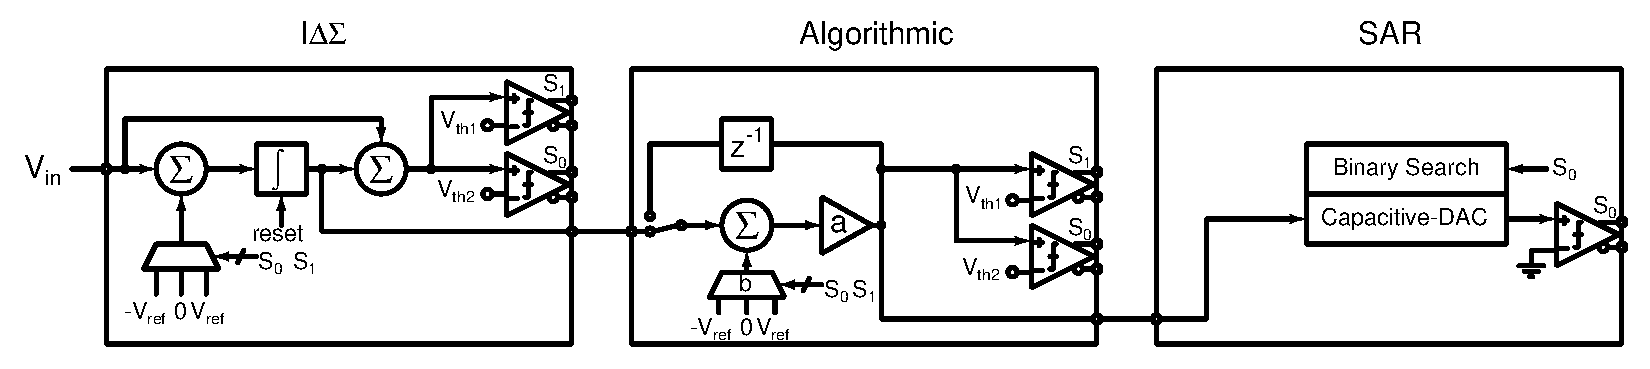
\includegraphics[width=\textwidth]{Chapter4/Figs/architecture-full-principle.ps}
        a) architecture originelle
        \vspace{2em}
    \end{minipage}
    \begin{minipage}[b]{\textwidth}
        \centering
        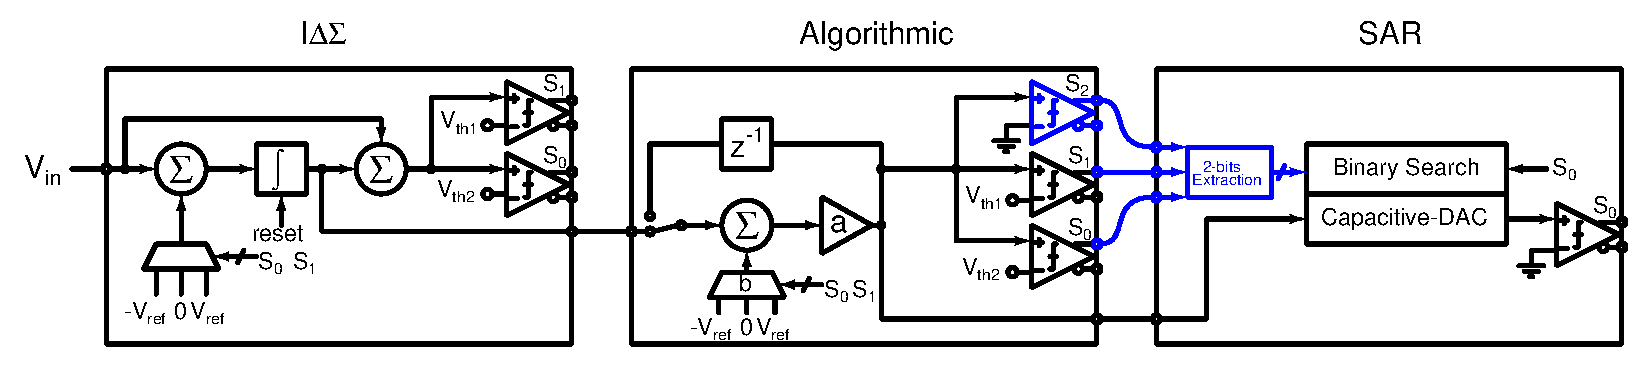
\includegraphics[width=\textwidth]{Chapter4/Figs/architecture-full-principle-final.ps}
        b) amélioration
    \end{minipage}
	\caption[]{Architecture hybride en trois étages et son amélioration pour ajouter un bit supplémentaire en minimisant la surface estimé en utilisant les derniers bits d'un convertisseur algorithmique comme premiers bits d'un SAR à redistribution de charge}
	\label{fig:final-prop-adc-architecture}
\end{center}
Fort de ceci, et des limitations en température qu'imposent les courants de fuites, des améliorations furent portées à l'architecture proposée. Dans un premier temps, un comparateur fut ajouté au sein de l'algorithmique. Ce dernier permet d'utiliser les derniers bits fournis au dernier coups d'horloge d'un échantillon, comme les deux premiers bits issus de la conversion du SAR\@. La répartition des bits est donc 3-4-5.5 au lieu de 3-5-3.5. Le bit supplémentaire fut dans un second temps utilisé pour rendre le SAR moins sensible aux mauvaises décisions venant de l'algorithmique et d'une génération des tensions de référence insuffisamment précise. En plus de cela, en changeant le radix, la sensibilité due aux courants de fuites est aussi diminuée puisqu'une redondance est introduite et que le pas du LSB est plus grand. Enfin, il fut envisagé d'améliorer encore la résolution pour un sur-échantillonnage de 6 coups d'horloge au lieu de 5. L'utilisation d'un coup d'horloge supplémentaire permet d'atteindre la résolution de 13.9-bits.

En plus de l'optimisation de l'architecture, le Chapitre~\ref{sec:adc-implementation} présente les mesures prises lors du dimensionnement et lors du layout en vue d'une répétabilité accrue pour une moindre surface.

La fiabilité ne fut pas laissé en reste même si le dernier étage emploie un design pseudo asynchrone afin de relâcher la contrainte de temps sur la prise de décision du comparateur dépendant de la température. Suivant une approche top-down, l'architecture fut d'abord validée par une simulation MATLAB puis Spice Haut niveau. Cette dernière nous a permis d'estimer plus précisément les spécifications des sous-blocs analogiques principaux en utilisant des modèles Verilog-AMS\@. Puis ces modèles furent remplacés par leur implémentation au niveau transistor, et par une netlist spice après extraction des parasites due au layout. Les performances statiques telles que la précision, le DNL, l'INL, \ldots sont le résultat d'un post-traitement MATLAB des simulations MATLAB et Spice.

Parmi l'ensemble des implémentations possibles décrit dans le début du chapitre~\ref{sec:analog-building-bloc}, les sous-blocs analogiques principaux choisis sont le Strong ARM, le Double-Tail, et le Gain-Boosted Complementary Folded Cascode. Dans l'état de l'art, les deux comparateurs choisis et leurs dérivés sont les plus utilisés actuellement. Bien que les équations de conception soient connues, leur sensibilité à la température l'est beaucoup moins. Les deux comparateurs sont donc analysés et comparés afin de choisir le plus approprié pour chaque étage du convertisseur pour une variation de 6$\sigma$ des paramètres du procédé de fabrication. Issu de ce travail, un nouveau modèle analytique pour le délai du Double-Tail fut présenté lors de l'ECCTD qui s'est tenu en 2017.

\begin{center}
    \centering
    \begin{minipage}[b]{0.33\textwidth}
        \centering
        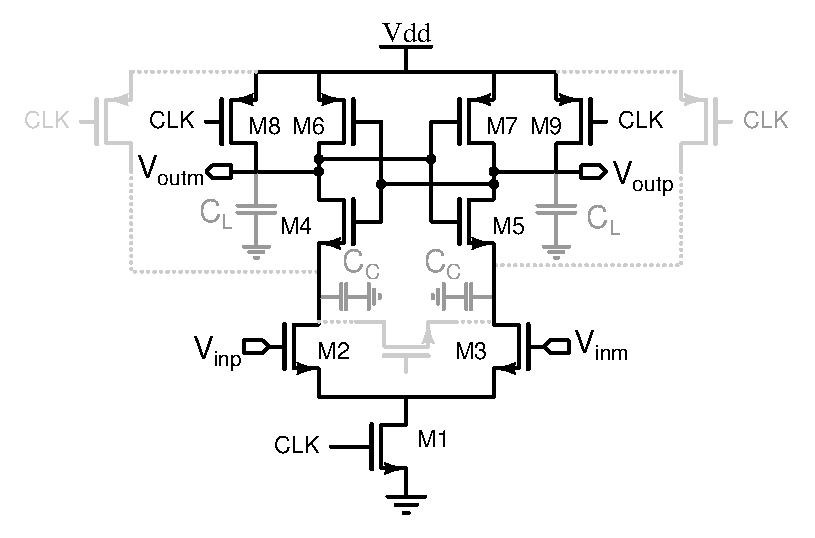
\includegraphics[width=\textwidth]{Abstract/Figs/sa_designed.eps}
        a) Strong-Arm latch
    \end{minipage}
    \begin{minipage}[b]{0.33\textwidth}
        \centering
        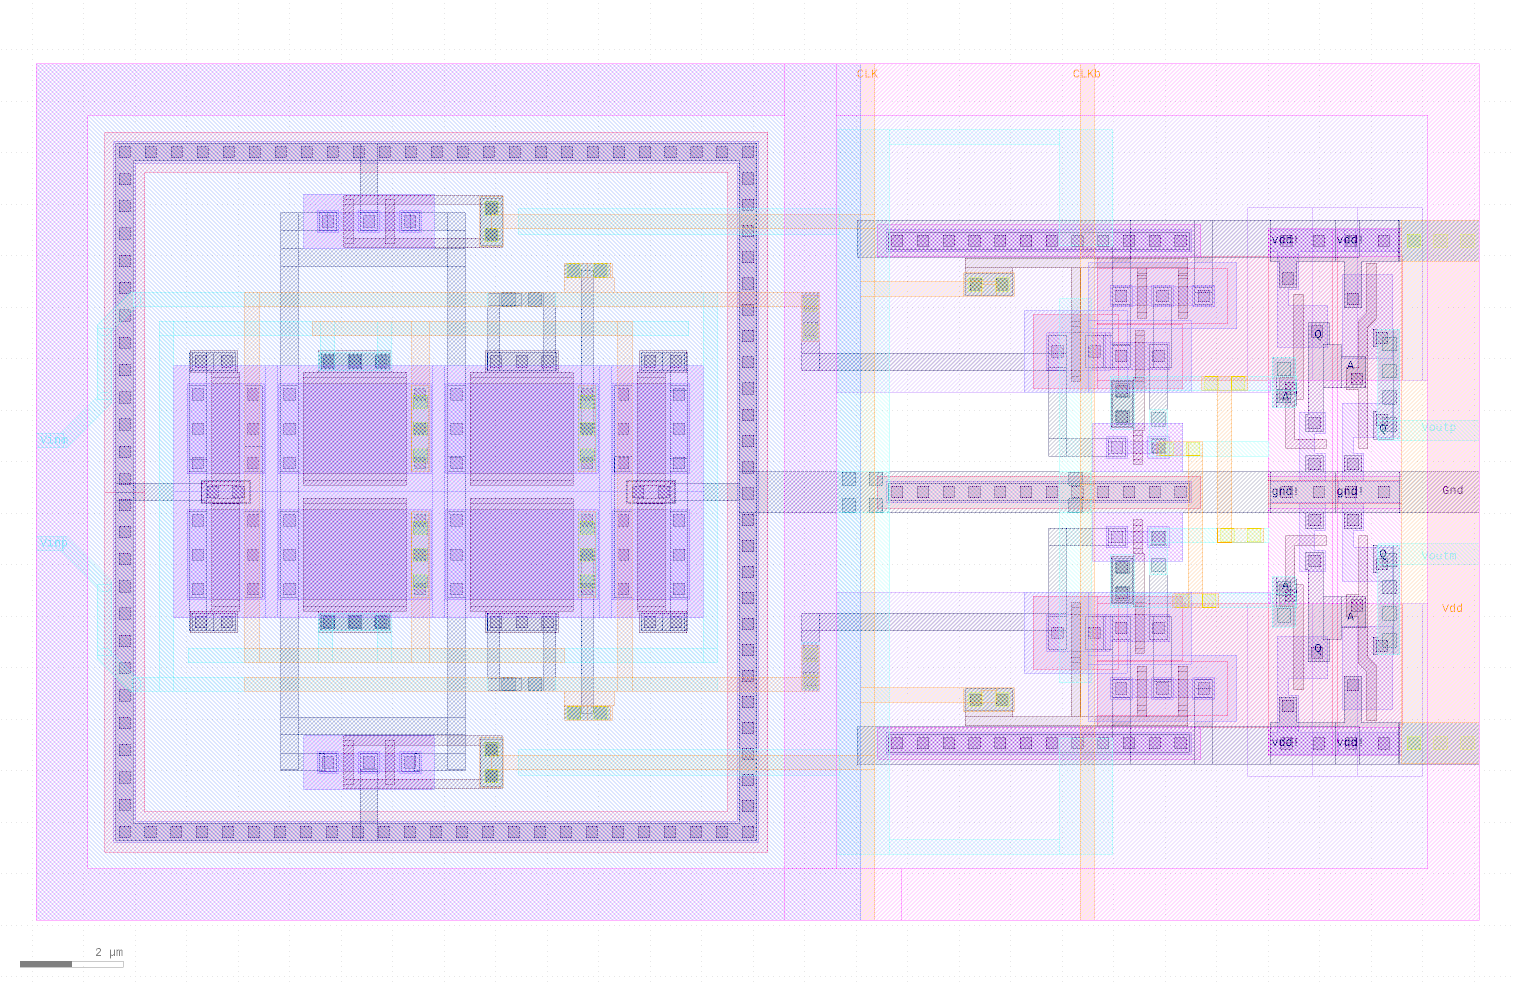
\includegraphics[width=\textwidth]{Chapter7/Figs/layout-slow-sa.png}
        b) Strong-Arm Layout
    \end{minipage}
    \begin{minipage}[b]{0.33\textwidth}
        \centering
        \resizebox {\textwidth} {!} { 
            %% Creator: Matplotlib, PGF backend
%%
%% To include the figure in your LaTeX document, write
%%   \input{<filename>.pgf}
%%
%% Make sure the required packages are loaded in your preamble
%%   \usepackage{pgf}
%%
%% Figures using additional raster images can only be included by \input if
%% they are in the same directory as the main LaTeX file. For loading figures
%% from other directories you can use the `import` package
%%   \usepackage{import}
%% and then include the figures with
%%   \import{<path to file>}{<filename>.pgf}
%%
%% Matplotlib used the following preamble
%%   \usepackage{gensymb}
%%   \usepackage[utf8x]{inputenc}
%%   \usepackage[T1]{fontenc}
%%
\begingroup%
\makeatletter%
\begin{pgfpicture}%
\pgfpathrectangle{\pgfpointorigin}{\pgfqpoint{2.961440in}{2.149917in}}%
\pgfusepath{use as bounding box, clip}%
\begin{pgfscope}%
\pgfsetbuttcap%
\pgfsetmiterjoin%
\definecolor{currentfill}{rgb}{1.000000,1.000000,1.000000}%
\pgfsetfillcolor{currentfill}%
\pgfsetlinewidth{0.000000pt}%
\definecolor{currentstroke}{rgb}{1.000000,1.000000,1.000000}%
\pgfsetstrokecolor{currentstroke}%
\pgfsetdash{}{0pt}%
\pgfpathmoveto{\pgfqpoint{-0.000000in}{0.000000in}}%
\pgfpathlineto{\pgfqpoint{2.961440in}{0.000000in}}%
\pgfpathlineto{\pgfqpoint{2.961440in}{2.149917in}}%
\pgfpathlineto{\pgfqpoint{-0.000000in}{2.149917in}}%
\pgfpathclose%
\pgfusepath{fill}%
\end{pgfscope}%
\begin{pgfscope}%
\pgfsetbuttcap%
\pgfsetmiterjoin%
\definecolor{currentfill}{rgb}{1.000000,1.000000,1.000000}%
\pgfsetfillcolor{currentfill}%
\pgfsetlinewidth{0.000000pt}%
\definecolor{currentstroke}{rgb}{0.000000,0.000000,0.000000}%
\pgfsetstrokecolor{currentstroke}%
\pgfsetstrokeopacity{0.000000}%
\pgfsetdash{}{0pt}%
\pgfpathmoveto{\pgfqpoint{0.541332in}{0.489099in}}%
\pgfpathlineto{\pgfqpoint{2.757273in}{0.489099in}}%
\pgfpathlineto{\pgfqpoint{2.757273in}{1.814584in}}%
\pgfpathlineto{\pgfqpoint{0.541332in}{1.814584in}}%
\pgfpathclose%
\pgfusepath{fill}%
\end{pgfscope}%
\begin{pgfscope}%
\pgfpathrectangle{\pgfqpoint{0.541332in}{0.489099in}}{\pgfqpoint{2.215942in}{1.325486in}} %
\pgfusepath{clip}%
\pgfsetbuttcap%
\pgfsetroundjoin%
\definecolor{currentfill}{rgb}{0.666667,0.223529,0.223529}%
\pgfsetfillcolor{currentfill}%
\pgfsetfillopacity{0.250000}%
\pgfsetlinewidth{0.000000pt}%
\definecolor{currentstroke}{rgb}{0.000000,0.000000,0.000000}%
\pgfsetstrokecolor{currentstroke}%
\pgfsetdash{}{0pt}%
\pgfpathmoveto{\pgfqpoint{0.541332in}{0.790117in}}%
\pgfpathlineto{\pgfqpoint{0.541332in}{0.558858in}}%
\pgfpathlineto{\pgfqpoint{0.695932in}{0.594521in}}%
\pgfpathlineto{\pgfqpoint{0.953600in}{0.631229in}}%
\pgfpathlineto{\pgfqpoint{1.211267in}{0.712948in}}%
\pgfpathlineto{\pgfqpoint{1.231881in}{0.729900in}}%
\pgfpathlineto{\pgfqpoint{1.592616in}{0.772133in}}%
\pgfpathlineto{\pgfqpoint{1.829670in}{0.872082in}}%
\pgfpathlineto{\pgfqpoint{1.984270in}{0.887719in}}%
\pgfpathlineto{\pgfqpoint{2.241938in}{0.915752in}}%
\pgfpathlineto{\pgfqpoint{2.499606in}{1.029181in}}%
\pgfpathlineto{\pgfqpoint{2.757273in}{1.096098in}}%
\pgfpathlineto{\pgfqpoint{2.757273in}{1.468401in}}%
\pgfpathlineto{\pgfqpoint{2.757273in}{1.468401in}}%
\pgfpathlineto{\pgfqpoint{2.499606in}{1.372654in}}%
\pgfpathlineto{\pgfqpoint{2.241938in}{1.347332in}}%
\pgfpathlineto{\pgfqpoint{1.984270in}{1.243041in}}%
\pgfpathlineto{\pgfqpoint{1.829670in}{1.156867in}}%
\pgfpathlineto{\pgfqpoint{1.592616in}{1.141353in}}%
\pgfpathlineto{\pgfqpoint{1.231881in}{0.996441in}}%
\pgfpathlineto{\pgfqpoint{1.211267in}{1.003969in}}%
\pgfpathlineto{\pgfqpoint{0.953600in}{0.947042in}}%
\pgfpathlineto{\pgfqpoint{0.695932in}{0.841592in}}%
\pgfpathlineto{\pgfqpoint{0.541332in}{0.790117in}}%
\pgfpathclose%
\pgfusepath{fill}%
\end{pgfscope}%
\begin{pgfscope}%
\pgfpathrectangle{\pgfqpoint{0.541332in}{0.489099in}}{\pgfqpoint{2.215942in}{1.325486in}} %
\pgfusepath{clip}%
\pgfsetbuttcap%
\pgfsetroundjoin%
\definecolor{currentfill}{rgb}{0.666667,0.592157,0.223529}%
\pgfsetfillcolor{currentfill}%
\pgfsetfillopacity{0.250000}%
\pgfsetlinewidth{0.000000pt}%
\definecolor{currentstroke}{rgb}{0.000000,0.000000,0.000000}%
\pgfsetstrokecolor{currentstroke}%
\pgfsetdash{}{0pt}%
\pgfpathmoveto{\pgfqpoint{0.541332in}{0.744268in}}%
\pgfpathlineto{\pgfqpoint{0.541332in}{0.509047in}}%
\pgfpathlineto{\pgfqpoint{0.695932in}{0.530451in}}%
\pgfpathlineto{\pgfqpoint{0.953600in}{0.598669in}}%
\pgfpathlineto{\pgfqpoint{1.211267in}{0.659006in}}%
\pgfpathlineto{\pgfqpoint{1.231881in}{0.654862in}}%
\pgfpathlineto{\pgfqpoint{1.592616in}{0.751820in}}%
\pgfpathlineto{\pgfqpoint{1.829670in}{0.791841in}}%
\pgfpathlineto{\pgfqpoint{1.984270in}{0.817652in}}%
\pgfpathlineto{\pgfqpoint{2.241938in}{0.890839in}}%
\pgfpathlineto{\pgfqpoint{2.499606in}{0.947627in}}%
\pgfpathlineto{\pgfqpoint{2.757273in}{0.989230in}}%
\pgfpathlineto{\pgfqpoint{2.757273in}{1.390588in}}%
\pgfpathlineto{\pgfqpoint{2.757273in}{1.390588in}}%
\pgfpathlineto{\pgfqpoint{2.499606in}{1.307437in}}%
\pgfpathlineto{\pgfqpoint{2.241938in}{1.254581in}}%
\pgfpathlineto{\pgfqpoint{1.984270in}{1.201900in}}%
\pgfpathlineto{\pgfqpoint{1.829670in}{1.144378in}}%
\pgfpathlineto{\pgfqpoint{1.592616in}{1.045170in}}%
\pgfpathlineto{\pgfqpoint{1.231881in}{0.964924in}}%
\pgfpathlineto{\pgfqpoint{1.211267in}{0.952229in}}%
\pgfpathlineto{\pgfqpoint{0.953600in}{0.879396in}}%
\pgfpathlineto{\pgfqpoint{0.695932in}{0.818020in}}%
\pgfpathlineto{\pgfqpoint{0.541332in}{0.744268in}}%
\pgfpathclose%
\pgfusepath{fill}%
\end{pgfscope}%
\begin{pgfscope}%
\pgfsetbuttcap%
\pgfsetroundjoin%
\definecolor{currentfill}{rgb}{0.000000,0.000000,0.000000}%
\pgfsetfillcolor{currentfill}%
\pgfsetlinewidth{0.803000pt}%
\definecolor{currentstroke}{rgb}{0.000000,0.000000,0.000000}%
\pgfsetstrokecolor{currentstroke}%
\pgfsetdash{}{0pt}%
\pgfsys@defobject{currentmarker}{\pgfqpoint{0.000000in}{-0.048611in}}{\pgfqpoint{0.000000in}{0.000000in}}{%
\pgfpathmoveto{\pgfqpoint{0.000000in}{0.000000in}}%
\pgfpathlineto{\pgfqpoint{0.000000in}{-0.048611in}}%
\pgfusepath{stroke,fill}%
}%
\begin{pgfscope}%
\pgfsys@transformshift{0.541332in}{0.489099in}%
\pgfsys@useobject{currentmarker}{}%
\end{pgfscope}%
\end{pgfscope}%
\begin{pgfscope}%
\pgftext[x=0.541332in,y=0.391876in,,top]{\fontsize{10.000000}{12.000000}\selectfont \(\displaystyle -40\)}%
\end{pgfscope}%
\begin{pgfscope}%
\pgfsetbuttcap%
\pgfsetroundjoin%
\definecolor{currentfill}{rgb}{0.000000,0.000000,0.000000}%
\pgfsetfillcolor{currentfill}%
\pgfsetlinewidth{0.803000pt}%
\definecolor{currentstroke}{rgb}{0.000000,0.000000,0.000000}%
\pgfsetstrokecolor{currentstroke}%
\pgfsetdash{}{0pt}%
\pgfsys@defobject{currentmarker}{\pgfqpoint{0.000000in}{-0.048611in}}{\pgfqpoint{0.000000in}{0.000000in}}{%
\pgfpathmoveto{\pgfqpoint{0.000000in}{0.000000in}}%
\pgfpathlineto{\pgfqpoint{0.000000in}{-0.048611in}}%
\pgfusepath{stroke,fill}%
}%
\begin{pgfscope}%
\pgfsys@transformshift{0.953600in}{0.489099in}%
\pgfsys@useobject{currentmarker}{}%
\end{pgfscope}%
\end{pgfscope}%
\begin{pgfscope}%
\pgftext[x=0.953600in,y=0.391876in,,top]{\fontsize{10.000000}{12.000000}\selectfont \(\displaystyle 0\)}%
\end{pgfscope}%
\begin{pgfscope}%
\pgfsetbuttcap%
\pgfsetroundjoin%
\definecolor{currentfill}{rgb}{0.000000,0.000000,0.000000}%
\pgfsetfillcolor{currentfill}%
\pgfsetlinewidth{0.803000pt}%
\definecolor{currentstroke}{rgb}{0.000000,0.000000,0.000000}%
\pgfsetstrokecolor{currentstroke}%
\pgfsetdash{}{0pt}%
\pgfsys@defobject{currentmarker}{\pgfqpoint{0.000000in}{-0.048611in}}{\pgfqpoint{0.000000in}{0.000000in}}{%
\pgfpathmoveto{\pgfqpoint{0.000000in}{0.000000in}}%
\pgfpathlineto{\pgfqpoint{0.000000in}{-0.048611in}}%
\pgfusepath{stroke,fill}%
}%
\begin{pgfscope}%
\pgfsys@transformshift{1.231881in}{0.489099in}%
\pgfsys@useobject{currentmarker}{}%
\end{pgfscope}%
\end{pgfscope}%
\begin{pgfscope}%
\pgftext[x=1.231881in,y=0.391876in,,top]{\fontsize{10.000000}{12.000000}\selectfont \(\displaystyle 27\)}%
\end{pgfscope}%
\begin{pgfscope}%
\pgfsetbuttcap%
\pgfsetroundjoin%
\definecolor{currentfill}{rgb}{0.000000,0.000000,0.000000}%
\pgfsetfillcolor{currentfill}%
\pgfsetlinewidth{0.803000pt}%
\definecolor{currentstroke}{rgb}{0.000000,0.000000,0.000000}%
\pgfsetstrokecolor{currentstroke}%
\pgfsetdash{}{0pt}%
\pgfsys@defobject{currentmarker}{\pgfqpoint{0.000000in}{-0.048611in}}{\pgfqpoint{0.000000in}{0.000000in}}{%
\pgfpathmoveto{\pgfqpoint{0.000000in}{0.000000in}}%
\pgfpathlineto{\pgfqpoint{0.000000in}{-0.048611in}}%
\pgfusepath{stroke,fill}%
}%
\begin{pgfscope}%
\pgfsys@transformshift{1.829670in}{0.489099in}%
\pgfsys@useobject{currentmarker}{}%
\end{pgfscope}%
\end{pgfscope}%
\begin{pgfscope}%
\pgftext[x=1.829670in,y=0.391876in,,top]{\fontsize{10.000000}{12.000000}\selectfont \(\displaystyle 85\)}%
\end{pgfscope}%
\begin{pgfscope}%
\pgfsetbuttcap%
\pgfsetroundjoin%
\definecolor{currentfill}{rgb}{0.000000,0.000000,0.000000}%
\pgfsetfillcolor{currentfill}%
\pgfsetlinewidth{0.803000pt}%
\definecolor{currentstroke}{rgb}{0.000000,0.000000,0.000000}%
\pgfsetstrokecolor{currentstroke}%
\pgfsetdash{}{0pt}%
\pgfsys@defobject{currentmarker}{\pgfqpoint{0.000000in}{-0.048611in}}{\pgfqpoint{0.000000in}{0.000000in}}{%
\pgfpathmoveto{\pgfqpoint{0.000000in}{0.000000in}}%
\pgfpathlineto{\pgfqpoint{0.000000in}{-0.048611in}}%
\pgfusepath{stroke,fill}%
}%
\begin{pgfscope}%
\pgfsys@transformshift{2.499606in}{0.489099in}%
\pgfsys@useobject{currentmarker}{}%
\end{pgfscope}%
\end{pgfscope}%
\begin{pgfscope}%
\pgftext[x=2.499606in,y=0.391876in,,top]{\fontsize{10.000000}{12.000000}\selectfont \(\displaystyle 150\)}%
\end{pgfscope}%
\begin{pgfscope}%
\pgfsetbuttcap%
\pgfsetroundjoin%
\definecolor{currentfill}{rgb}{0.000000,0.000000,0.000000}%
\pgfsetfillcolor{currentfill}%
\pgfsetlinewidth{0.803000pt}%
\definecolor{currentstroke}{rgb}{0.000000,0.000000,0.000000}%
\pgfsetstrokecolor{currentstroke}%
\pgfsetdash{}{0pt}%
\pgfsys@defobject{currentmarker}{\pgfqpoint{0.000000in}{-0.048611in}}{\pgfqpoint{0.000000in}{0.000000in}}{%
\pgfpathmoveto{\pgfqpoint{0.000000in}{0.000000in}}%
\pgfpathlineto{\pgfqpoint{0.000000in}{-0.048611in}}%
\pgfusepath{stroke,fill}%
}%
\begin{pgfscope}%
\pgfsys@transformshift{2.757273in}{0.489099in}%
\pgfsys@useobject{currentmarker}{}%
\end{pgfscope}%
\end{pgfscope}%
\begin{pgfscope}%
\pgftext[x=2.757273in,y=0.391876in,,top]{\fontsize{10.000000}{12.000000}\selectfont \(\displaystyle 175\)}%
\end{pgfscope}%
\begin{pgfscope}%
\pgftext[x=1.649302in,y=0.213666in,,top]{\fontsize{8.000000}{9.600000}\selectfont Temperature [\(\displaystyle \degree\)C]}%
\end{pgfscope}%
\begin{pgfscope}%
\pgfsetbuttcap%
\pgfsetroundjoin%
\definecolor{currentfill}{rgb}{0.000000,0.000000,0.000000}%
\pgfsetfillcolor{currentfill}%
\pgfsetlinewidth{0.803000pt}%
\definecolor{currentstroke}{rgb}{0.000000,0.000000,0.000000}%
\pgfsetstrokecolor{currentstroke}%
\pgfsetdash{}{0pt}%
\pgfsys@defobject{currentmarker}{\pgfqpoint{-0.048611in}{0.000000in}}{\pgfqpoint{0.000000in}{0.000000in}}{%
\pgfpathmoveto{\pgfqpoint{0.000000in}{0.000000in}}%
\pgfpathlineto{\pgfqpoint{-0.048611in}{0.000000in}}%
\pgfusepath{stroke,fill}%
}%
\begin{pgfscope}%
\pgfsys@transformshift{0.541332in}{0.489099in}%
\pgfsys@useobject{currentmarker}{}%
\end{pgfscope}%
\end{pgfscope}%
\begin{pgfscope}%
\pgftext[x=0.266640in,y=0.441271in,left,base]{\fontsize{10.000000}{12.000000}\selectfont \(\displaystyle 1.5\)}%
\end{pgfscope}%
\begin{pgfscope}%
\pgfsetbuttcap%
\pgfsetroundjoin%
\definecolor{currentfill}{rgb}{0.000000,0.000000,0.000000}%
\pgfsetfillcolor{currentfill}%
\pgfsetlinewidth{0.803000pt}%
\definecolor{currentstroke}{rgb}{0.000000,0.000000,0.000000}%
\pgfsetstrokecolor{currentstroke}%
\pgfsetdash{}{0pt}%
\pgfsys@defobject{currentmarker}{\pgfqpoint{-0.048611in}{0.000000in}}{\pgfqpoint{0.000000in}{0.000000in}}{%
\pgfpathmoveto{\pgfqpoint{0.000000in}{0.000000in}}%
\pgfpathlineto{\pgfqpoint{-0.048611in}{0.000000in}}%
\pgfusepath{stroke,fill}%
}%
\begin{pgfscope}%
\pgfsys@transformshift{0.541332in}{0.820470in}%
\pgfsys@useobject{currentmarker}{}%
\end{pgfscope}%
\end{pgfscope}%
\begin{pgfscope}%
\pgftext[x=0.266640in,y=0.772642in,left,base]{\fontsize{10.000000}{12.000000}\selectfont \(\displaystyle 2.0\)}%
\end{pgfscope}%
\begin{pgfscope}%
\pgfsetbuttcap%
\pgfsetroundjoin%
\definecolor{currentfill}{rgb}{0.000000,0.000000,0.000000}%
\pgfsetfillcolor{currentfill}%
\pgfsetlinewidth{0.803000pt}%
\definecolor{currentstroke}{rgb}{0.000000,0.000000,0.000000}%
\pgfsetstrokecolor{currentstroke}%
\pgfsetdash{}{0pt}%
\pgfsys@defobject{currentmarker}{\pgfqpoint{-0.048611in}{0.000000in}}{\pgfqpoint{0.000000in}{0.000000in}}{%
\pgfpathmoveto{\pgfqpoint{0.000000in}{0.000000in}}%
\pgfpathlineto{\pgfqpoint{-0.048611in}{0.000000in}}%
\pgfusepath{stroke,fill}%
}%
\begin{pgfscope}%
\pgfsys@transformshift{0.541332in}{1.151841in}%
\pgfsys@useobject{currentmarker}{}%
\end{pgfscope}%
\end{pgfscope}%
\begin{pgfscope}%
\pgftext[x=0.266640in,y=1.104014in,left,base]{\fontsize{10.000000}{12.000000}\selectfont \(\displaystyle 2.5\)}%
\end{pgfscope}%
\begin{pgfscope}%
\pgfsetbuttcap%
\pgfsetroundjoin%
\definecolor{currentfill}{rgb}{0.000000,0.000000,0.000000}%
\pgfsetfillcolor{currentfill}%
\pgfsetlinewidth{0.803000pt}%
\definecolor{currentstroke}{rgb}{0.000000,0.000000,0.000000}%
\pgfsetstrokecolor{currentstroke}%
\pgfsetdash{}{0pt}%
\pgfsys@defobject{currentmarker}{\pgfqpoint{-0.048611in}{0.000000in}}{\pgfqpoint{0.000000in}{0.000000in}}{%
\pgfpathmoveto{\pgfqpoint{0.000000in}{0.000000in}}%
\pgfpathlineto{\pgfqpoint{-0.048611in}{0.000000in}}%
\pgfusepath{stroke,fill}%
}%
\begin{pgfscope}%
\pgfsys@transformshift{0.541332in}{1.483213in}%
\pgfsys@useobject{currentmarker}{}%
\end{pgfscope}%
\end{pgfscope}%
\begin{pgfscope}%
\pgftext[x=0.266640in,y=1.435385in,left,base]{\fontsize{10.000000}{12.000000}\selectfont \(\displaystyle 3.0\)}%
\end{pgfscope}%
\begin{pgfscope}%
\pgfsetbuttcap%
\pgfsetroundjoin%
\definecolor{currentfill}{rgb}{0.000000,0.000000,0.000000}%
\pgfsetfillcolor{currentfill}%
\pgfsetlinewidth{0.803000pt}%
\definecolor{currentstroke}{rgb}{0.000000,0.000000,0.000000}%
\pgfsetstrokecolor{currentstroke}%
\pgfsetdash{}{0pt}%
\pgfsys@defobject{currentmarker}{\pgfqpoint{-0.048611in}{0.000000in}}{\pgfqpoint{0.000000in}{0.000000in}}{%
\pgfpathmoveto{\pgfqpoint{0.000000in}{0.000000in}}%
\pgfpathlineto{\pgfqpoint{-0.048611in}{0.000000in}}%
\pgfusepath{stroke,fill}%
}%
\begin{pgfscope}%
\pgfsys@transformshift{0.541332in}{1.814584in}%
\pgfsys@useobject{currentmarker}{}%
\end{pgfscope}%
\end{pgfscope}%
\begin{pgfscope}%
\pgftext[x=0.266640in,y=1.766756in,left,base]{\fontsize{10.000000}{12.000000}\selectfont \(\displaystyle 3.5\)}%
\end{pgfscope}%
\begin{pgfscope}%
\pgftext[x=0.211084in,y=1.151841in,,bottom,rotate=90.000000]{\fontsize{8.000000}{9.600000}\selectfont Time Delay [ns]}%
\end{pgfscope}%
\begin{pgfscope}%
\pgfpathrectangle{\pgfqpoint{0.541332in}{0.489099in}}{\pgfqpoint{2.215942in}{1.325486in}} %
\pgfusepath{clip}%
\pgfsetrectcap%
\pgfsetroundjoin%
\pgfsetlinewidth{2.007500pt}%
\definecolor{currentstroke}{rgb}{0.666667,0.223529,0.223529}%
\pgfsetstrokecolor{currentstroke}%
\pgfsetdash{}{0pt}%
\pgfpathmoveto{\pgfqpoint{0.541332in}{0.674488in}}%
\pgfpathlineto{\pgfqpoint{0.695932in}{0.718056in}}%
\pgfpathlineto{\pgfqpoint{0.953600in}{0.789136in}}%
\pgfpathlineto{\pgfqpoint{1.211267in}{0.858458in}}%
\pgfpathlineto{\pgfqpoint{1.231881in}{0.863171in}}%
\pgfpathlineto{\pgfqpoint{1.592616in}{0.956743in}}%
\pgfpathlineto{\pgfqpoint{1.829670in}{1.014475in}}%
\pgfpathlineto{\pgfqpoint{1.984270in}{1.065380in}}%
\pgfpathlineto{\pgfqpoint{2.241938in}{1.131542in}}%
\pgfpathlineto{\pgfqpoint{2.499606in}{1.200918in}}%
\pgfpathlineto{\pgfqpoint{2.757273in}{1.282249in}}%
\pgfusepath{stroke}%
\end{pgfscope}%
\begin{pgfscope}%
\pgfpathrectangle{\pgfqpoint{0.541332in}{0.489099in}}{\pgfqpoint{2.215942in}{1.325486in}} %
\pgfusepath{clip}%
\pgfsetrectcap%
\pgfsetroundjoin%
\pgfsetlinewidth{2.007500pt}%
\definecolor{currentstroke}{rgb}{0.666667,0.592157,0.223529}%
\pgfsetstrokecolor{currentstroke}%
\pgfsetdash{}{0pt}%
\pgfpathmoveto{\pgfqpoint{0.541332in}{0.626658in}}%
\pgfpathlineto{\pgfqpoint{0.695932in}{0.674236in}}%
\pgfpathlineto{\pgfqpoint{0.953600in}{0.739032in}}%
\pgfpathlineto{\pgfqpoint{1.211267in}{0.805618in}}%
\pgfpathlineto{\pgfqpoint{1.231881in}{0.809893in}}%
\pgfpathlineto{\pgfqpoint{1.592616in}{0.898495in}}%
\pgfpathlineto{\pgfqpoint{1.829670in}{0.968109in}}%
\pgfpathlineto{\pgfqpoint{1.984270in}{1.009776in}}%
\pgfpathlineto{\pgfqpoint{2.241938in}{1.072710in}}%
\pgfpathlineto{\pgfqpoint{2.499606in}{1.127532in}}%
\pgfpathlineto{\pgfqpoint{2.757273in}{1.189909in}}%
\pgfusepath{stroke}%
\end{pgfscope}%
\begin{pgfscope}%
\pgfsetrectcap%
\pgfsetmiterjoin%
\pgfsetlinewidth{0.803000pt}%
\definecolor{currentstroke}{rgb}{0.000000,0.000000,0.000000}%
\pgfsetstrokecolor{currentstroke}%
\pgfsetdash{}{0pt}%
\pgfpathmoveto{\pgfqpoint{0.541332in}{0.489099in}}%
\pgfpathlineto{\pgfqpoint{0.541332in}{1.814584in}}%
\pgfusepath{stroke}%
\end{pgfscope}%
\begin{pgfscope}%
\pgfsetrectcap%
\pgfsetmiterjoin%
\pgfsetlinewidth{0.803000pt}%
\definecolor{currentstroke}{rgb}{0.000000,0.000000,0.000000}%
\pgfsetstrokecolor{currentstroke}%
\pgfsetdash{}{0pt}%
\pgfpathmoveto{\pgfqpoint{2.757273in}{0.489099in}}%
\pgfpathlineto{\pgfqpoint{2.757273in}{1.814584in}}%
\pgfusepath{stroke}%
\end{pgfscope}%
\begin{pgfscope}%
\pgfsetrectcap%
\pgfsetmiterjoin%
\pgfsetlinewidth{0.803000pt}%
\definecolor{currentstroke}{rgb}{0.000000,0.000000,0.000000}%
\pgfsetstrokecolor{currentstroke}%
\pgfsetdash{}{0pt}%
\pgfpathmoveto{\pgfqpoint{0.541332in}{0.489099in}}%
\pgfpathlineto{\pgfqpoint{2.757273in}{0.489099in}}%
\pgfusepath{stroke}%
\end{pgfscope}%
\begin{pgfscope}%
\pgfsetrectcap%
\pgfsetmiterjoin%
\pgfsetlinewidth{0.803000pt}%
\definecolor{currentstroke}{rgb}{0.000000,0.000000,0.000000}%
\pgfsetstrokecolor{currentstroke}%
\pgfsetdash{}{0pt}%
\pgfpathmoveto{\pgfqpoint{0.541332in}{1.814584in}}%
\pgfpathlineto{\pgfqpoint{2.757273in}{1.814584in}}%
\pgfusepath{stroke}%
\end{pgfscope}%
\begin{pgfscope}%
\pgfsetbuttcap%
\pgfsetmiterjoin%
\definecolor{currentfill}{rgb}{1.000000,1.000000,1.000000}%
\pgfsetfillcolor{currentfill}%
\pgfsetfillopacity{0.800000}%
\pgfsetlinewidth{1.003750pt}%
\definecolor{currentstroke}{rgb}{0.800000,0.800000,0.800000}%
\pgfsetstrokecolor{currentstroke}%
\pgfsetstrokeopacity{0.800000}%
\pgfsetdash{}{0pt}%
\pgfpathmoveto{\pgfqpoint{0.591269in}{1.814584in}}%
\pgfpathlineto{\pgfqpoint{2.751655in}{1.814584in}}%
\pgfpathquadraticcurveto{\pgfqpoint{2.779433in}{1.814584in}}{\pgfqpoint{2.779433in}{1.842362in}}%
\pgfpathlineto{\pgfqpoint{2.779433in}{2.022139in}}%
\pgfpathquadraticcurveto{\pgfqpoint{2.779433in}{2.049917in}}{\pgfqpoint{2.751655in}{2.049917in}}%
\pgfpathlineto{\pgfqpoint{0.591269in}{2.049917in}}%
\pgfpathquadraticcurveto{\pgfqpoint{0.563491in}{2.049917in}}{\pgfqpoint{0.563491in}{2.022139in}}%
\pgfpathlineto{\pgfqpoint{0.563491in}{1.842362in}}%
\pgfpathquadraticcurveto{\pgfqpoint{0.563491in}{1.814584in}}{\pgfqpoint{0.591269in}{1.814584in}}%
\pgfpathclose%
\pgfusepath{stroke,fill}%
\end{pgfscope}%
\begin{pgfscope}%
\pgfsetrectcap%
\pgfsetroundjoin%
\pgfsetlinewidth{2.007500pt}%
\definecolor{currentstroke}{rgb}{0.666667,0.223529,0.223529}%
\pgfsetstrokecolor{currentstroke}%
\pgfsetdash{}{0pt}%
\pgfpathmoveto{\pgfqpoint{0.619047in}{1.945750in}}%
\pgfpathlineto{\pgfqpoint{0.757935in}{1.945750in}}%
\pgfusepath{stroke}%
\end{pgfscope}%
\begin{pgfscope}%
\pgftext[x=0.869047in,y=1.897139in,left,base]{\fontsize{10.000000}{12.000000}\selectfont Double Tail}%
\end{pgfscope}%
\begin{pgfscope}%
\pgfsetrectcap%
\pgfsetroundjoin%
\pgfsetlinewidth{2.007500pt}%
\definecolor{currentstroke}{rgb}{0.666667,0.592157,0.223529}%
\pgfsetstrokecolor{currentstroke}%
\pgfsetdash{}{0pt}%
\pgfpathmoveto{\pgfqpoint{1.692432in}{1.945750in}}%
\pgfpathlineto{\pgfqpoint{1.831321in}{1.945750in}}%
\pgfusepath{stroke}%
\end{pgfscope}%
\begin{pgfscope}%
\pgftext[x=1.942432in,y=1.897139in,left,base]{\fontsize{10.000000}{12.000000}\selectfont Strong ARM}%
\end{pgfscope}%
\end{pgfpicture}%
\makeatother%
\endgroup%

        }
        c) temps de reponse
    \end{minipage}
    \begin{minipage}[b]{0.33\textwidth}
        \centering
        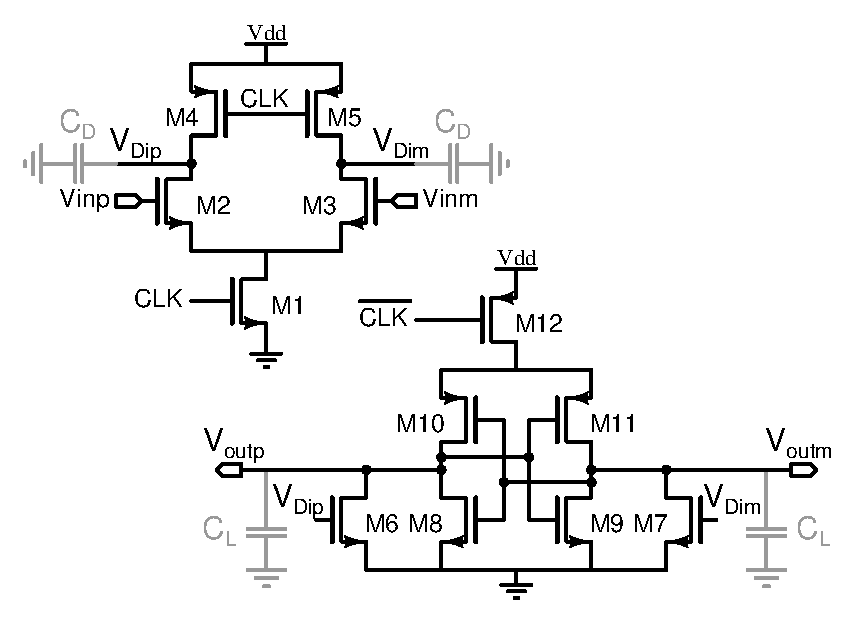
\includegraphics[width=\textwidth]{Abstract/Figs/dtl_designed.eps}
        d) Double-Tail latch
    \end{minipage}
    \begin{minipage}[b]{0.33\textwidth}
        \centering
        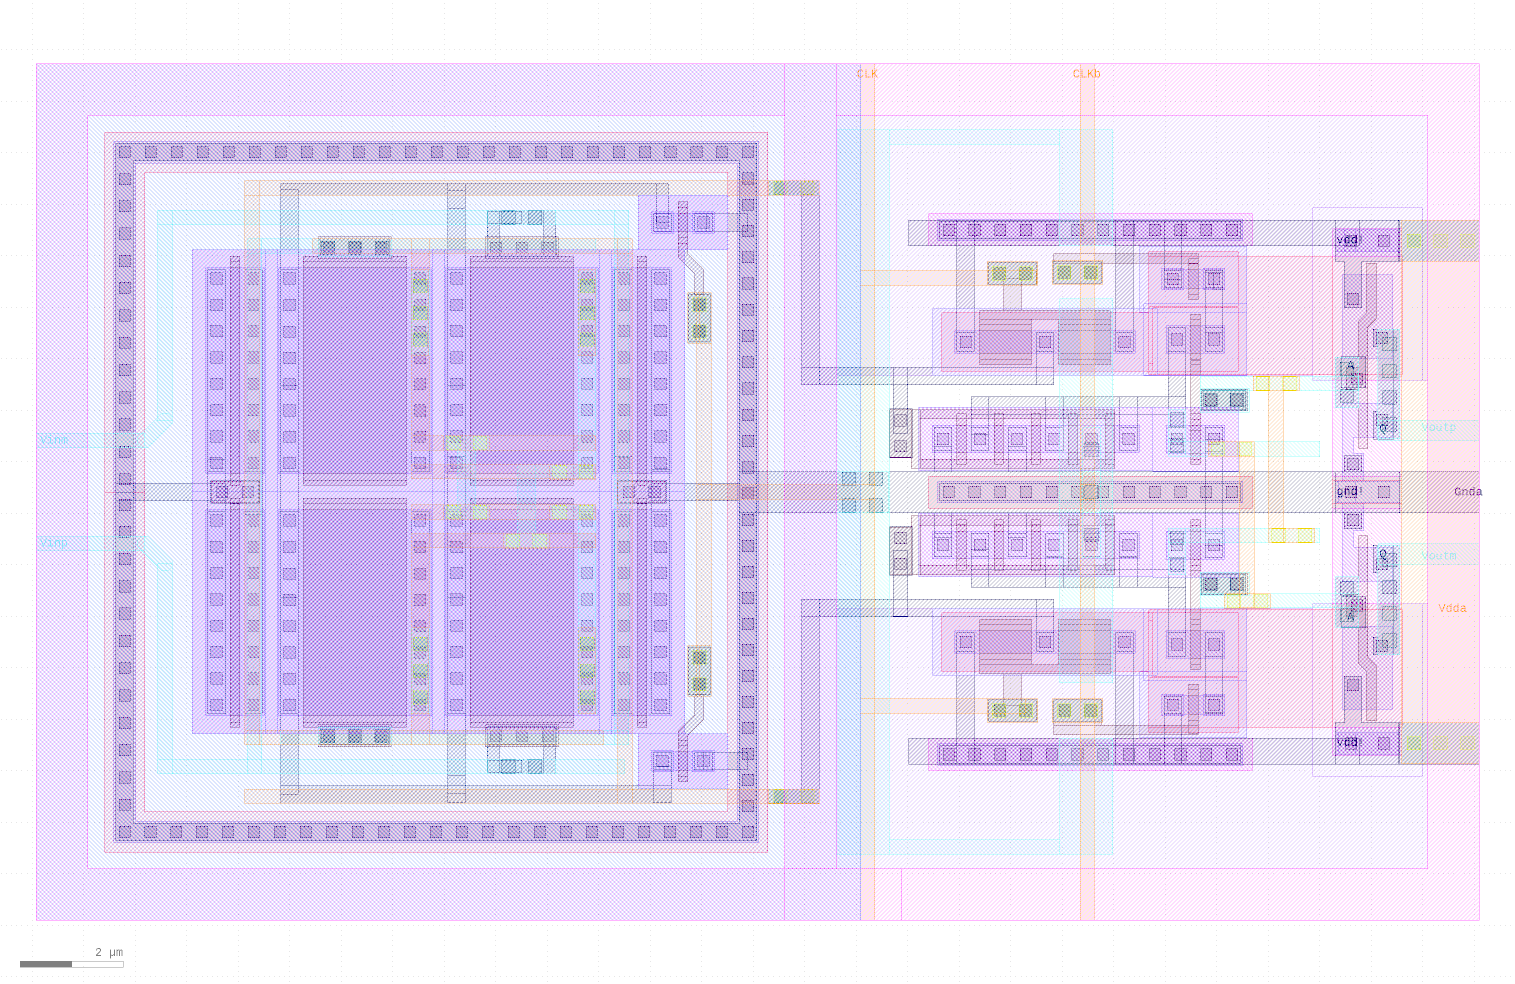
\includegraphics[width=\textwidth]{Chapter7/Figs/layout-slow-dtl.png}
        e) Double-Tail Layout
    \end{minipage}
    \begin{minipage}[b]{0.33\textwidth}
        \centering
        \resizebox {\textwidth} {!} { 
            %% Creator: Matplotlib, PGF backend
%%
%% To include the figure in your LaTeX document, write
%%   \input{<filename>.pgf}
%%
%% Make sure the required packages are loaded in your preamble
%%   \usepackage{pgf}
%%
%% Figures using additional raster images can only be included by \input if
%% they are in the same directory as the main LaTeX file. For loading figures
%% from other directories you can use the `import` package
%%   \usepackage{import}
%% and then include the figures with
%%   \import{<path to file>}{<filename>.pgf}
%%
%% Matplotlib used the following preamble
%%   \usepackage{gensymb}
%%   \usepackage[utf8x]{inputenc}
%%   \usepackage[T1]{fontenc}
%%
\begingroup%
\makeatletter%
\begin{pgfpicture}%
\pgfpathrectangle{\pgfpointorigin}{\pgfqpoint{2.960907in}{1.962629in}}%
\pgfusepath{use as bounding box, clip}%
\begin{pgfscope}%
\pgfsetbuttcap%
\pgfsetmiterjoin%
\definecolor{currentfill}{rgb}{1.000000,1.000000,1.000000}%
\pgfsetfillcolor{currentfill}%
\pgfsetlinewidth{0.000000pt}%
\definecolor{currentstroke}{rgb}{1.000000,1.000000,1.000000}%
\pgfsetstrokecolor{currentstroke}%
\pgfsetdash{}{0pt}%
\pgfpathmoveto{\pgfqpoint{0.000000in}{0.000000in}}%
\pgfpathlineto{\pgfqpoint{2.960907in}{0.000000in}}%
\pgfpathlineto{\pgfqpoint{2.960907in}{1.962629in}}%
\pgfpathlineto{\pgfqpoint{0.000000in}{1.962629in}}%
\pgfpathclose%
\pgfusepath{fill}%
\end{pgfscope}%
\begin{pgfscope}%
\pgfsetbuttcap%
\pgfsetmiterjoin%
\definecolor{currentfill}{rgb}{1.000000,1.000000,1.000000}%
\pgfsetfillcolor{currentfill}%
\pgfsetlinewidth{0.000000pt}%
\definecolor{currentstroke}{rgb}{0.000000,0.000000,0.000000}%
\pgfsetstrokecolor{currentstroke}%
\pgfsetstrokeopacity{0.000000}%
\pgfsetdash{}{0pt}%
\pgfpathmoveto{\pgfqpoint{0.502751in}{0.489099in}}%
\pgfpathlineto{\pgfqpoint{2.843407in}{0.489099in}}%
\pgfpathlineto{\pgfqpoint{2.843407in}{1.845129in}}%
\pgfpathlineto{\pgfqpoint{0.502751in}{1.845129in}}%
\pgfpathclose%
\pgfusepath{fill}%
\end{pgfscope}%
\begin{pgfscope}%
\pgfpathrectangle{\pgfqpoint{0.502751in}{0.489099in}}{\pgfqpoint{2.340656in}{1.356031in}} %
\pgfusepath{clip}%
\pgfsetbuttcap%
\pgfsetroundjoin%
\definecolor{currentfill}{rgb}{0.666667,0.223529,0.223529}%
\pgfsetfillcolor{currentfill}%
\pgfsetfillopacity{0.250000}%
\pgfsetlinewidth{0.000000pt}%
\definecolor{currentstroke}{rgb}{0.000000,0.000000,0.000000}%
\pgfsetstrokecolor{currentstroke}%
\pgfsetdash{}{0pt}%
\pgfpathmoveto{\pgfqpoint{0.609145in}{1.503744in}}%
\pgfpathlineto{\pgfqpoint{0.609145in}{1.387254in}}%
\pgfpathlineto{\pgfqpoint{0.757601in}{1.405740in}}%
\pgfpathlineto{\pgfqpoint{1.005027in}{1.435241in}}%
\pgfpathlineto{\pgfqpoint{1.252454in}{1.463566in}}%
\pgfpathlineto{\pgfqpoint{1.272248in}{1.465817in}}%
\pgfpathlineto{\pgfqpoint{1.618645in}{1.504158in}}%
\pgfpathlineto{\pgfqpoint{1.846278in}{1.528490in}}%
\pgfpathlineto{\pgfqpoint{1.994734in}{1.544066in}}%
\pgfpathlineto{\pgfqpoint{2.242160in}{1.569703in}}%
\pgfpathlineto{\pgfqpoint{2.489587in}{1.595896in}}%
\pgfpathlineto{\pgfqpoint{2.737013in}{1.622345in}}%
\pgfpathlineto{\pgfqpoint{2.737013in}{1.783492in}}%
\pgfpathlineto{\pgfqpoint{2.737013in}{1.783492in}}%
\pgfpathlineto{\pgfqpoint{2.489587in}{1.750872in}}%
\pgfpathlineto{\pgfqpoint{2.242160in}{1.719203in}}%
\pgfpathlineto{\pgfqpoint{1.994734in}{1.687829in}}%
\pgfpathlineto{\pgfqpoint{1.846278in}{1.669290in}}%
\pgfpathlineto{\pgfqpoint{1.618645in}{1.640583in}}%
\pgfpathlineto{\pgfqpoint{1.272248in}{1.595413in}}%
\pgfpathlineto{\pgfqpoint{1.252454in}{1.592834in}}%
\pgfpathlineto{\pgfqpoint{1.005027in}{1.559628in}}%
\pgfpathlineto{\pgfqpoint{0.757601in}{1.525241in}}%
\pgfpathlineto{\pgfqpoint{0.609145in}{1.503744in}}%
\pgfpathclose%
\pgfusepath{fill}%
\end{pgfscope}%
\begin{pgfscope}%
\pgfpathrectangle{\pgfqpoint{0.502751in}{0.489099in}}{\pgfqpoint{2.340656in}{1.356031in}} %
\pgfusepath{clip}%
\pgfsetbuttcap%
\pgfsetroundjoin%
\definecolor{currentfill}{rgb}{0.666667,0.592157,0.223529}%
\pgfsetfillcolor{currentfill}%
\pgfsetfillopacity{0.250000}%
\pgfsetlinewidth{0.000000pt}%
\definecolor{currentstroke}{rgb}{0.000000,0.000000,0.000000}%
\pgfsetstrokecolor{currentstroke}%
\pgfsetdash{}{0pt}%
\pgfpathmoveto{\pgfqpoint{0.609145in}{0.590992in}}%
\pgfpathlineto{\pgfqpoint{0.609145in}{0.550736in}}%
\pgfpathlineto{\pgfqpoint{0.757601in}{0.556399in}}%
\pgfpathlineto{\pgfqpoint{1.005027in}{0.565761in}}%
\pgfpathlineto{\pgfqpoint{1.252454in}{0.574833in}}%
\pgfpathlineto{\pgfqpoint{1.272248in}{0.575602in}}%
\pgfpathlineto{\pgfqpoint{1.618645in}{0.588298in}}%
\pgfpathlineto{\pgfqpoint{1.846278in}{0.596913in}}%
\pgfpathlineto{\pgfqpoint{1.994734in}{0.602113in}}%
\pgfpathlineto{\pgfqpoint{2.242160in}{0.610845in}}%
\pgfpathlineto{\pgfqpoint{2.489587in}{0.619662in}}%
\pgfpathlineto{\pgfqpoint{2.737013in}{0.628351in}}%
\pgfpathlineto{\pgfqpoint{2.737013in}{0.674901in}}%
\pgfpathlineto{\pgfqpoint{2.737013in}{0.674901in}}%
\pgfpathlineto{\pgfqpoint{2.489587in}{0.665061in}}%
\pgfpathlineto{\pgfqpoint{2.242160in}{0.655173in}}%
\pgfpathlineto{\pgfqpoint{1.994734in}{0.645309in}}%
\pgfpathlineto{\pgfqpoint{1.846278in}{0.639448in}}%
\pgfpathlineto{\pgfqpoint{1.618645in}{0.630637in}}%
\pgfpathlineto{\pgfqpoint{1.272248in}{0.617224in}}%
\pgfpathlineto{\pgfqpoint{1.252454in}{0.616469in}}%
\pgfpathlineto{\pgfqpoint{1.005027in}{0.606626in}}%
\pgfpathlineto{\pgfqpoint{0.757601in}{0.596846in}}%
\pgfpathlineto{\pgfqpoint{0.609145in}{0.590992in}}%
\pgfpathclose%
\pgfusepath{fill}%
\end{pgfscope}%
\begin{pgfscope}%
\pgfsetbuttcap%
\pgfsetroundjoin%
\definecolor{currentfill}{rgb}{0.000000,0.000000,0.000000}%
\pgfsetfillcolor{currentfill}%
\pgfsetlinewidth{0.803000pt}%
\definecolor{currentstroke}{rgb}{0.000000,0.000000,0.000000}%
\pgfsetstrokecolor{currentstroke}%
\pgfsetdash{}{0pt}%
\pgfsys@defobject{currentmarker}{\pgfqpoint{0.000000in}{-0.048611in}}{\pgfqpoint{0.000000in}{0.000000in}}{%
\pgfpathmoveto{\pgfqpoint{0.000000in}{0.000000in}}%
\pgfpathlineto{\pgfqpoint{0.000000in}{-0.048611in}}%
\pgfusepath{stroke,fill}%
}%
\begin{pgfscope}%
\pgfsys@transformshift{0.609145in}{0.489099in}%
\pgfsys@useobject{currentmarker}{}%
\end{pgfscope}%
\end{pgfscope}%
\begin{pgfscope}%
\pgftext[x=0.609145in,y=0.391876in,,top]{\fontsize{10.000000}{12.000000}\selectfont \(\displaystyle -40\)}%
\end{pgfscope}%
\begin{pgfscope}%
\pgfsetbuttcap%
\pgfsetroundjoin%
\definecolor{currentfill}{rgb}{0.000000,0.000000,0.000000}%
\pgfsetfillcolor{currentfill}%
\pgfsetlinewidth{0.803000pt}%
\definecolor{currentstroke}{rgb}{0.000000,0.000000,0.000000}%
\pgfsetstrokecolor{currentstroke}%
\pgfsetdash{}{0pt}%
\pgfsys@defobject{currentmarker}{\pgfqpoint{0.000000in}{-0.048611in}}{\pgfqpoint{0.000000in}{0.000000in}}{%
\pgfpathmoveto{\pgfqpoint{0.000000in}{0.000000in}}%
\pgfpathlineto{\pgfqpoint{0.000000in}{-0.048611in}}%
\pgfusepath{stroke,fill}%
}%
\begin{pgfscope}%
\pgfsys@transformshift{1.005027in}{0.489099in}%
\pgfsys@useobject{currentmarker}{}%
\end{pgfscope}%
\end{pgfscope}%
\begin{pgfscope}%
\pgftext[x=1.005027in,y=0.391876in,,top]{\fontsize{10.000000}{12.000000}\selectfont \(\displaystyle 0\)}%
\end{pgfscope}%
\begin{pgfscope}%
\pgfsetbuttcap%
\pgfsetroundjoin%
\definecolor{currentfill}{rgb}{0.000000,0.000000,0.000000}%
\pgfsetfillcolor{currentfill}%
\pgfsetlinewidth{0.803000pt}%
\definecolor{currentstroke}{rgb}{0.000000,0.000000,0.000000}%
\pgfsetstrokecolor{currentstroke}%
\pgfsetdash{}{0pt}%
\pgfsys@defobject{currentmarker}{\pgfqpoint{0.000000in}{-0.048611in}}{\pgfqpoint{0.000000in}{0.000000in}}{%
\pgfpathmoveto{\pgfqpoint{0.000000in}{0.000000in}}%
\pgfpathlineto{\pgfqpoint{0.000000in}{-0.048611in}}%
\pgfusepath{stroke,fill}%
}%
\begin{pgfscope}%
\pgfsys@transformshift{1.272248in}{0.489099in}%
\pgfsys@useobject{currentmarker}{}%
\end{pgfscope}%
\end{pgfscope}%
\begin{pgfscope}%
\pgftext[x=1.272248in,y=0.391876in,,top]{\fontsize{10.000000}{12.000000}\selectfont \(\displaystyle 27\)}%
\end{pgfscope}%
\begin{pgfscope}%
\pgfsetbuttcap%
\pgfsetroundjoin%
\definecolor{currentfill}{rgb}{0.000000,0.000000,0.000000}%
\pgfsetfillcolor{currentfill}%
\pgfsetlinewidth{0.803000pt}%
\definecolor{currentstroke}{rgb}{0.000000,0.000000,0.000000}%
\pgfsetstrokecolor{currentstroke}%
\pgfsetdash{}{0pt}%
\pgfsys@defobject{currentmarker}{\pgfqpoint{0.000000in}{-0.048611in}}{\pgfqpoint{0.000000in}{0.000000in}}{%
\pgfpathmoveto{\pgfqpoint{0.000000in}{0.000000in}}%
\pgfpathlineto{\pgfqpoint{0.000000in}{-0.048611in}}%
\pgfusepath{stroke,fill}%
}%
\begin{pgfscope}%
\pgfsys@transformshift{1.846278in}{0.489099in}%
\pgfsys@useobject{currentmarker}{}%
\end{pgfscope}%
\end{pgfscope}%
\begin{pgfscope}%
\pgftext[x=1.846278in,y=0.391876in,,top]{\fontsize{10.000000}{12.000000}\selectfont \(\displaystyle 85\)}%
\end{pgfscope}%
\begin{pgfscope}%
\pgfsetbuttcap%
\pgfsetroundjoin%
\definecolor{currentfill}{rgb}{0.000000,0.000000,0.000000}%
\pgfsetfillcolor{currentfill}%
\pgfsetlinewidth{0.803000pt}%
\definecolor{currentstroke}{rgb}{0.000000,0.000000,0.000000}%
\pgfsetstrokecolor{currentstroke}%
\pgfsetdash{}{0pt}%
\pgfsys@defobject{currentmarker}{\pgfqpoint{0.000000in}{-0.048611in}}{\pgfqpoint{0.000000in}{0.000000in}}{%
\pgfpathmoveto{\pgfqpoint{0.000000in}{0.000000in}}%
\pgfpathlineto{\pgfqpoint{0.000000in}{-0.048611in}}%
\pgfusepath{stroke,fill}%
}%
\begin{pgfscope}%
\pgfsys@transformshift{2.489587in}{0.489099in}%
\pgfsys@useobject{currentmarker}{}%
\end{pgfscope}%
\end{pgfscope}%
\begin{pgfscope}%
\pgftext[x=2.489587in,y=0.391876in,,top]{\fontsize{10.000000}{12.000000}\selectfont \(\displaystyle 150\)}%
\end{pgfscope}%
\begin{pgfscope}%
\pgfsetbuttcap%
\pgfsetroundjoin%
\definecolor{currentfill}{rgb}{0.000000,0.000000,0.000000}%
\pgfsetfillcolor{currentfill}%
\pgfsetlinewidth{0.803000pt}%
\definecolor{currentstroke}{rgb}{0.000000,0.000000,0.000000}%
\pgfsetstrokecolor{currentstroke}%
\pgfsetdash{}{0pt}%
\pgfsys@defobject{currentmarker}{\pgfqpoint{0.000000in}{-0.048611in}}{\pgfqpoint{0.000000in}{0.000000in}}{%
\pgfpathmoveto{\pgfqpoint{0.000000in}{0.000000in}}%
\pgfpathlineto{\pgfqpoint{0.000000in}{-0.048611in}}%
\pgfusepath{stroke,fill}%
}%
\begin{pgfscope}%
\pgfsys@transformshift{2.737013in}{0.489099in}%
\pgfsys@useobject{currentmarker}{}%
\end{pgfscope}%
\end{pgfscope}%
\begin{pgfscope}%
\pgftext[x=2.737013in,y=0.391876in,,top]{\fontsize{10.000000}{12.000000}\selectfont \(\displaystyle 175\)}%
\end{pgfscope}%
\begin{pgfscope}%
\pgftext[x=1.673079in,y=0.213666in,,top]{\fontsize{8.000000}{9.600000}\selectfont Temperature [\(\displaystyle \degree\)C]}%
\end{pgfscope}%
\begin{pgfscope}%
\pgfsetbuttcap%
\pgfsetroundjoin%
\definecolor{currentfill}{rgb}{0.000000,0.000000,0.000000}%
\pgfsetfillcolor{currentfill}%
\pgfsetlinewidth{0.803000pt}%
\definecolor{currentstroke}{rgb}{0.000000,0.000000,0.000000}%
\pgfsetstrokecolor{currentstroke}%
\pgfsetdash{}{0pt}%
\pgfsys@defobject{currentmarker}{\pgfqpoint{-0.048611in}{0.000000in}}{\pgfqpoint{0.000000in}{0.000000in}}{%
\pgfpathmoveto{\pgfqpoint{0.000000in}{0.000000in}}%
\pgfpathlineto{\pgfqpoint{-0.048611in}{0.000000in}}%
\pgfusepath{stroke,fill}%
}%
\begin{pgfscope}%
\pgfsys@transformshift{0.502751in}{0.789907in}%
\pgfsys@useobject{currentmarker}{}%
\end{pgfscope}%
\end{pgfscope}%
\begin{pgfscope}%
\pgftext[x=0.266640in,y=0.742079in,left,base]{\fontsize{10.000000}{12.000000}\selectfont \(\displaystyle 40\)}%
\end{pgfscope}%
\begin{pgfscope}%
\pgfsetbuttcap%
\pgfsetroundjoin%
\definecolor{currentfill}{rgb}{0.000000,0.000000,0.000000}%
\pgfsetfillcolor{currentfill}%
\pgfsetlinewidth{0.803000pt}%
\definecolor{currentstroke}{rgb}{0.000000,0.000000,0.000000}%
\pgfsetstrokecolor{currentstroke}%
\pgfsetdash{}{0pt}%
\pgfsys@defobject{currentmarker}{\pgfqpoint{-0.048611in}{0.000000in}}{\pgfqpoint{0.000000in}{0.000000in}}{%
\pgfpathmoveto{\pgfqpoint{0.000000in}{0.000000in}}%
\pgfpathlineto{\pgfqpoint{-0.048611in}{0.000000in}}%
\pgfusepath{stroke,fill}%
}%
\begin{pgfscope}%
\pgfsys@transformshift{0.502751in}{1.166119in}%
\pgfsys@useobject{currentmarker}{}%
\end{pgfscope}%
\end{pgfscope}%
\begin{pgfscope}%
\pgftext[x=0.266640in,y=1.118292in,left,base]{\fontsize{10.000000}{12.000000}\selectfont \(\displaystyle 60\)}%
\end{pgfscope}%
\begin{pgfscope}%
\pgfsetbuttcap%
\pgfsetroundjoin%
\definecolor{currentfill}{rgb}{0.000000,0.000000,0.000000}%
\pgfsetfillcolor{currentfill}%
\pgfsetlinewidth{0.803000pt}%
\definecolor{currentstroke}{rgb}{0.000000,0.000000,0.000000}%
\pgfsetstrokecolor{currentstroke}%
\pgfsetdash{}{0pt}%
\pgfsys@defobject{currentmarker}{\pgfqpoint{-0.048611in}{0.000000in}}{\pgfqpoint{0.000000in}{0.000000in}}{%
\pgfpathmoveto{\pgfqpoint{0.000000in}{0.000000in}}%
\pgfpathlineto{\pgfqpoint{-0.048611in}{0.000000in}}%
\pgfusepath{stroke,fill}%
}%
\begin{pgfscope}%
\pgfsys@transformshift{0.502751in}{1.542332in}%
\pgfsys@useobject{currentmarker}{}%
\end{pgfscope}%
\end{pgfscope}%
\begin{pgfscope}%
\pgftext[x=0.266640in,y=1.494504in,left,base]{\fontsize{10.000000}{12.000000}\selectfont \(\displaystyle 80\)}%
\end{pgfscope}%
\begin{pgfscope}%
\pgftext[x=0.211084in,y=1.167114in,,bottom,rotate=90.000000]{\fontsize{8.000000}{9.600000}\selectfont Average Power [\(\displaystyle \mu\)W]}%
\end{pgfscope}%
\begin{pgfscope}%
\pgfpathrectangle{\pgfqpoint{0.502751in}{0.489099in}}{\pgfqpoint{2.340656in}{1.356031in}} %
\pgfusepath{clip}%
\pgfsetrectcap%
\pgfsetroundjoin%
\pgfsetlinewidth{2.007500pt}%
\definecolor{currentstroke}{rgb}{0.666667,0.223529,0.223529}%
\pgfsetstrokecolor{currentstroke}%
\pgfsetdash{}{0pt}%
\pgfpathmoveto{\pgfqpoint{0.609145in}{1.445499in}}%
\pgfpathlineto{\pgfqpoint{0.757601in}{1.465491in}}%
\pgfpathlineto{\pgfqpoint{1.005027in}{1.497435in}}%
\pgfpathlineto{\pgfqpoint{1.252454in}{1.528200in}}%
\pgfpathlineto{\pgfqpoint{1.272248in}{1.530615in}}%
\pgfpathlineto{\pgfqpoint{1.618645in}{1.572371in}}%
\pgfpathlineto{\pgfqpoint{1.846278in}{1.598890in}}%
\pgfpathlineto{\pgfqpoint{1.994734in}{1.615947in}}%
\pgfpathlineto{\pgfqpoint{2.242160in}{1.644453in}}%
\pgfpathlineto{\pgfqpoint{2.489587in}{1.673384in}}%
\pgfpathlineto{\pgfqpoint{2.737013in}{1.702918in}}%
\pgfusepath{stroke}%
\end{pgfscope}%
\begin{pgfscope}%
\pgfpathrectangle{\pgfqpoint{0.502751in}{0.489099in}}{\pgfqpoint{2.340656in}{1.356031in}} %
\pgfusepath{clip}%
\pgfsetrectcap%
\pgfsetroundjoin%
\pgfsetlinewidth{2.007500pt}%
\definecolor{currentstroke}{rgb}{0.666667,0.592157,0.223529}%
\pgfsetstrokecolor{currentstroke}%
\pgfsetdash{}{0pt}%
\pgfpathmoveto{\pgfqpoint{0.609145in}{0.570864in}}%
\pgfpathlineto{\pgfqpoint{0.757601in}{0.576622in}}%
\pgfpathlineto{\pgfqpoint{1.005027in}{0.586193in}}%
\pgfpathlineto{\pgfqpoint{1.252454in}{0.595651in}}%
\pgfpathlineto{\pgfqpoint{1.272248in}{0.596413in}}%
\pgfpathlineto{\pgfqpoint{1.618645in}{0.609468in}}%
\pgfpathlineto{\pgfqpoint{1.846278in}{0.618181in}}%
\pgfpathlineto{\pgfqpoint{1.994734in}{0.623711in}}%
\pgfpathlineto{\pgfqpoint{2.242160in}{0.633009in}}%
\pgfpathlineto{\pgfqpoint{2.489587in}{0.642362in}}%
\pgfpathlineto{\pgfqpoint{2.737013in}{0.651626in}}%
\pgfusepath{stroke}%
\end{pgfscope}%
\begin{pgfscope}%
\pgfsetrectcap%
\pgfsetmiterjoin%
\pgfsetlinewidth{0.803000pt}%
\definecolor{currentstroke}{rgb}{0.000000,0.000000,0.000000}%
\pgfsetstrokecolor{currentstroke}%
\pgfsetdash{}{0pt}%
\pgfpathmoveto{\pgfqpoint{0.502751in}{0.489099in}}%
\pgfpathlineto{\pgfqpoint{0.502751in}{1.845129in}}%
\pgfusepath{stroke}%
\end{pgfscope}%
\begin{pgfscope}%
\pgfsetrectcap%
\pgfsetmiterjoin%
\pgfsetlinewidth{0.803000pt}%
\definecolor{currentstroke}{rgb}{0.000000,0.000000,0.000000}%
\pgfsetstrokecolor{currentstroke}%
\pgfsetdash{}{0pt}%
\pgfpathmoveto{\pgfqpoint{2.843407in}{0.489099in}}%
\pgfpathlineto{\pgfqpoint{2.843407in}{1.845129in}}%
\pgfusepath{stroke}%
\end{pgfscope}%
\begin{pgfscope}%
\pgfsetrectcap%
\pgfsetmiterjoin%
\pgfsetlinewidth{0.803000pt}%
\definecolor{currentstroke}{rgb}{0.000000,0.000000,0.000000}%
\pgfsetstrokecolor{currentstroke}%
\pgfsetdash{}{0pt}%
\pgfpathmoveto{\pgfqpoint{0.502751in}{0.489099in}}%
\pgfpathlineto{\pgfqpoint{2.843407in}{0.489099in}}%
\pgfusepath{stroke}%
\end{pgfscope}%
\begin{pgfscope}%
\pgfsetrectcap%
\pgfsetmiterjoin%
\pgfsetlinewidth{0.803000pt}%
\definecolor{currentstroke}{rgb}{0.000000,0.000000,0.000000}%
\pgfsetstrokecolor{currentstroke}%
\pgfsetdash{}{0pt}%
\pgfpathmoveto{\pgfqpoint{0.502751in}{1.845129in}}%
\pgfpathlineto{\pgfqpoint{2.843407in}{1.845129in}}%
\pgfusepath{stroke}%
\end{pgfscope}%
\end{pgfpicture}%
\makeatother%
\endgroup%

        }
        f) consommation
    \end{minipage}
    \caption[]{Comparateurs conçu pour la température}
\end{center}

Quant à l'amplificateur, si l'on considère un processus en 180 nm, la plupart des publications ont été publiées entre 2001 et 2008. Sur cette période, le Folded-Cascode, les OTA à deux étages, et ceux basées sur du gain-Boosting sont légion avec une préférence pour un Folded Cascode suivi par un étage en source-follower pour améliorer l'excursion de sortie. Pour des raisons de rapidité et de stabilité, le gain-boosting d'un OTA de classe AB fut privilégié. Les choix de conception et les contraintes liées au layout, représenté à la \figurename~\ref{fig:ota-fr}, sont aussi discutés dans ce chapitre. En matière de bruit, l'OTA génère un bruit maximum estimé de 198 \(\mu V _{rms} \) correspondant à 82\% du LSB d'un 12-bit sur l'excursion du résidu du premier étage. La consommation en courant n'excédant pas 1.8 mA, la consommation moyenne totale de l'analogique est estimée à 7 mW avec un maximum admis à -40 $\degree$C dans le corner FF de 14 mW.

\begin{center}
    \centering
    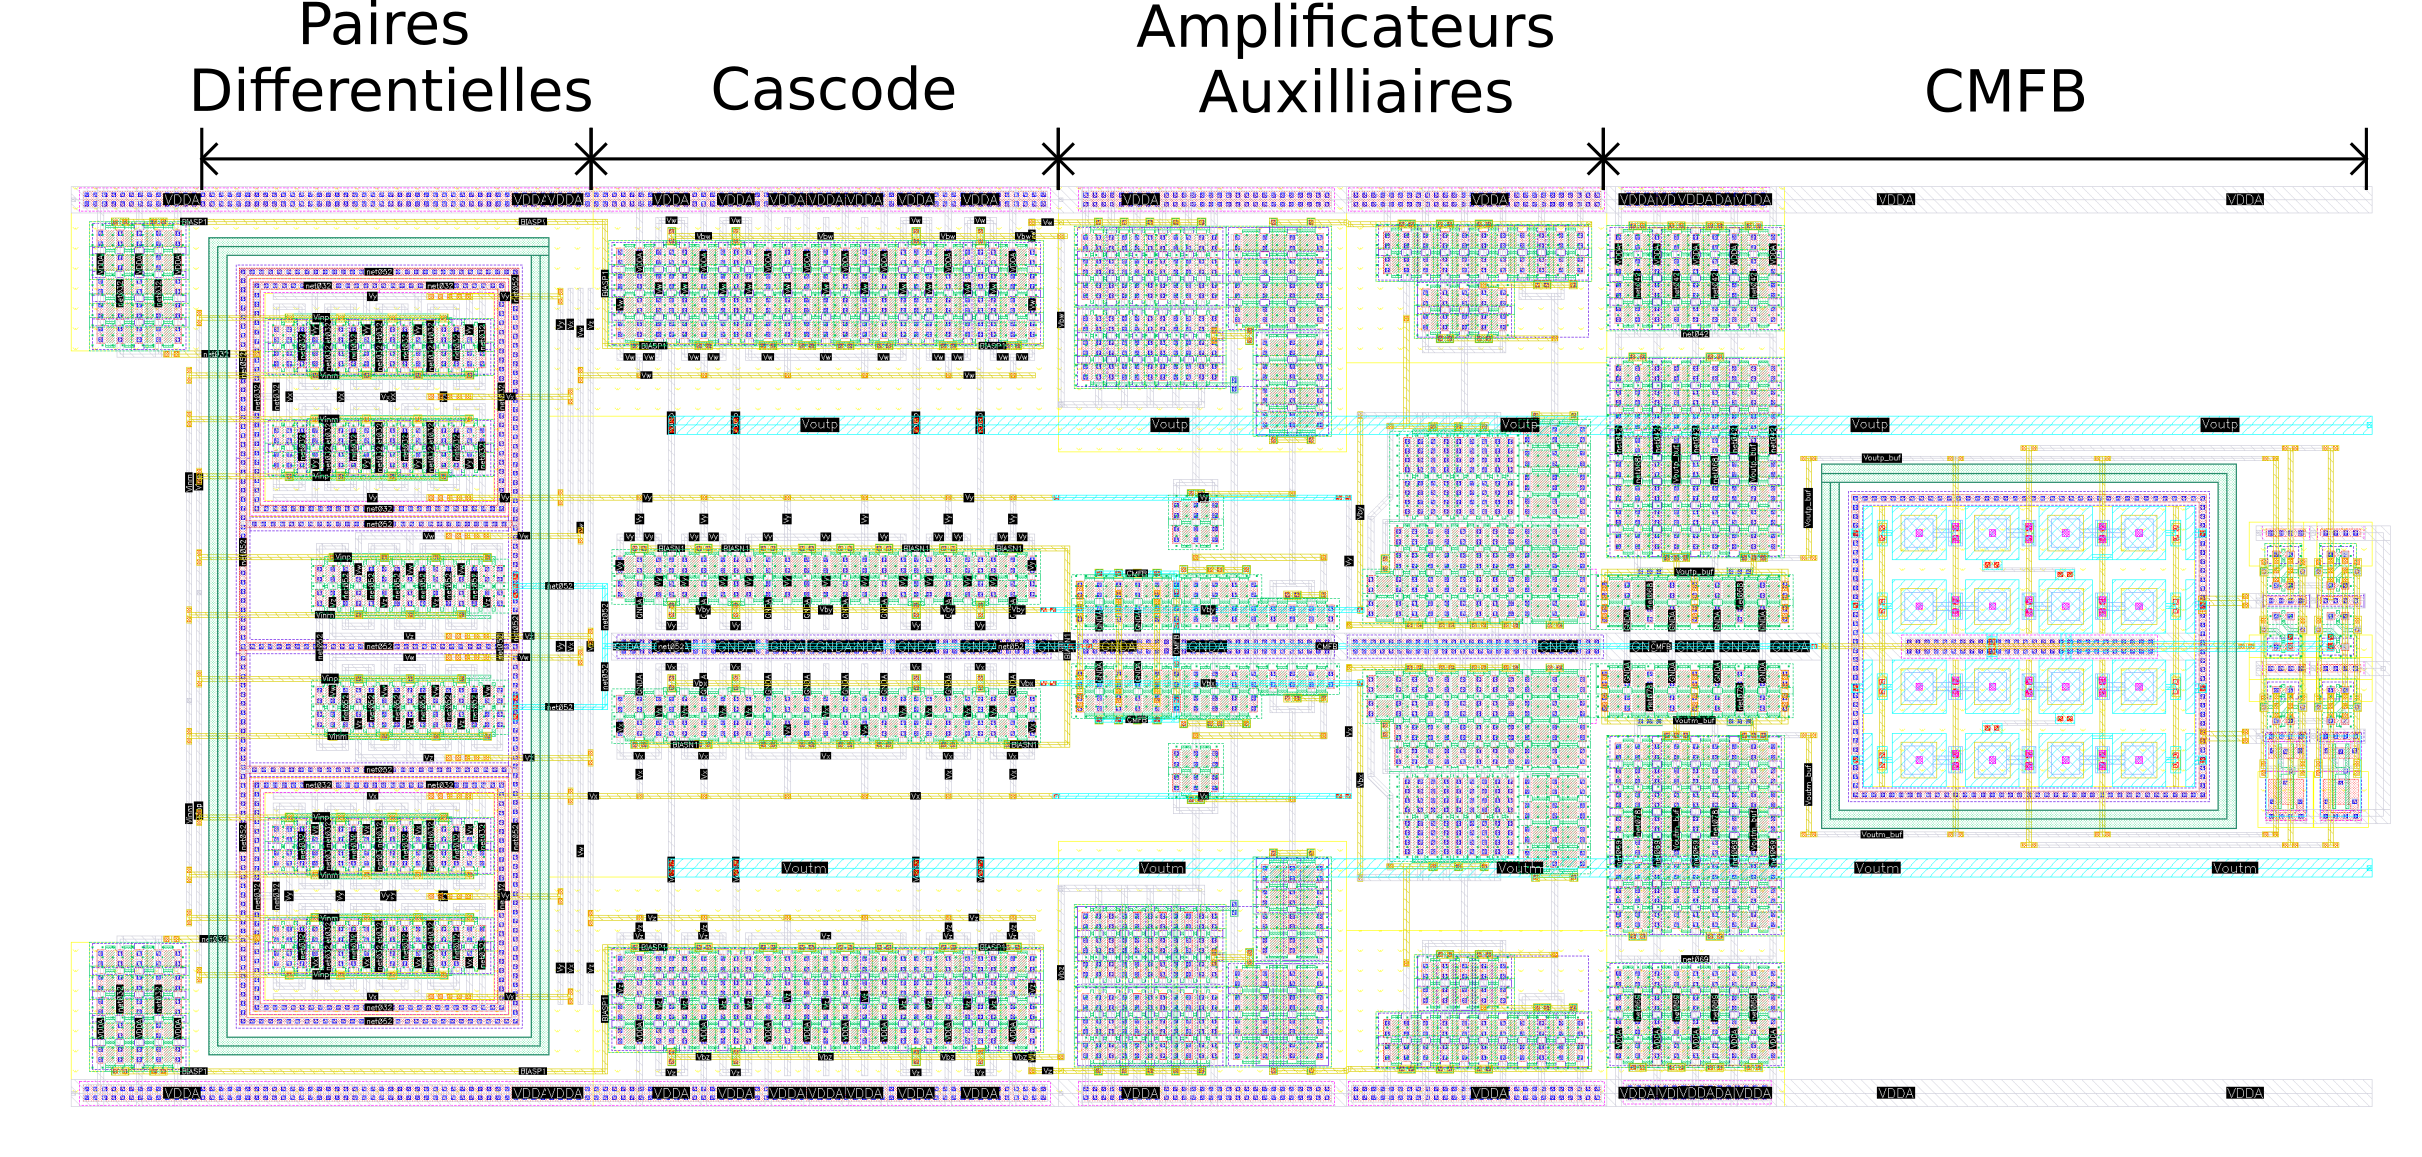
\includegraphics[width=0.65\textwidth]{Chapter7/Figs/layout_ota_v2-fr.png}
    \caption[]{Dessin de l'OTA conçu de dimension \(52 \mu m \times 128 \mu m\) avec une double pair différentielle interdigitée et common-centroid}
    \label{fig:ota-fr}
\end{center}

Étant donnée la polyvalence souhaitée du convertisseur et en vue de sa réutilisation, chaque élément de sa composition est validé expérimentalement. Ainsi, trois puces de test différentes furent conçues et présentées dans le chapitre~\ref{sec:tests-meas}. La première permet de valider le délai, l'offset, le bruit, l’hystérésis des comparateurs. Au cours de sa conception, un circuit de mesure du délai des comparateurs synchrones fut présenté lors de l'ECCTD 2017. Les résultats en température obtenus pour ce circuit s'accordent avec le modèle du délai pur et démontrent de bonnes performances en raison de sa taille en comparaison des circuits existant tel que dépeint à la \figurename~\ref{fig:meas_circ_schem-fr}. La seconde puce valide le fonctionnement pseudo asynchrone et les performances statiques du SAR en température. Suite aux améliorations de l'architecture, la testabilité du dernier étage se complexifie. Les procédures de test s'en trouvent donc modifiées et sont présentées. Le SAR démontre en température une importante stabilité de la pondération de chaque bit. Ce résultat permet donc de réutiliser cet étage pour la calibration des précédents, comme de réduire le temps de test de cet étage. Enfin, la dernière puce permet de valider chaque étage indépendamment et le convertisseur dans sa globalité. Cette dernière n'est pas encore envoyée en fonderie, et par conséquent, seulement la conception et les principes des tests à effectuer sont discutés.

\begin{center}
    \centering
    \begin{minipage}[b]{0.30\linewidth}
        \centering
        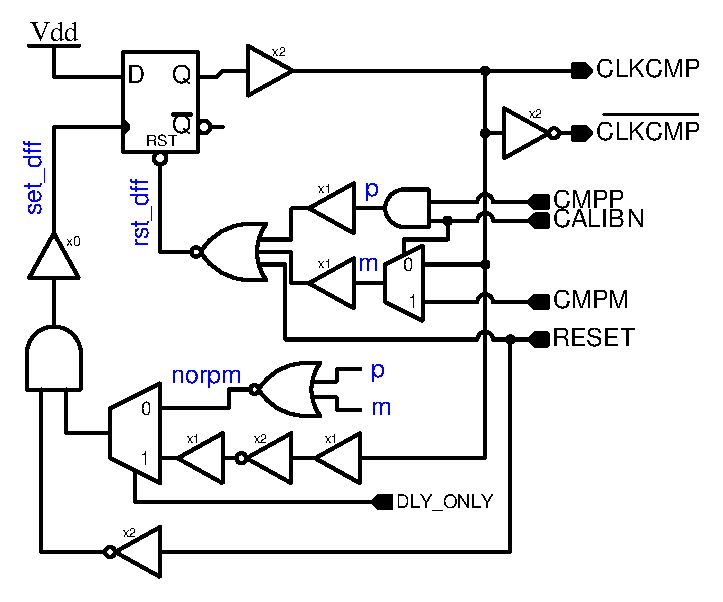
\includegraphics[width=\textwidth]{Chapter5/Figs/test_delay_comp_new_simp.ps}
        a) Schematique
    \end{minipage}
    \begin{minipage}[b]{0.38\linewidth}
        \centering
        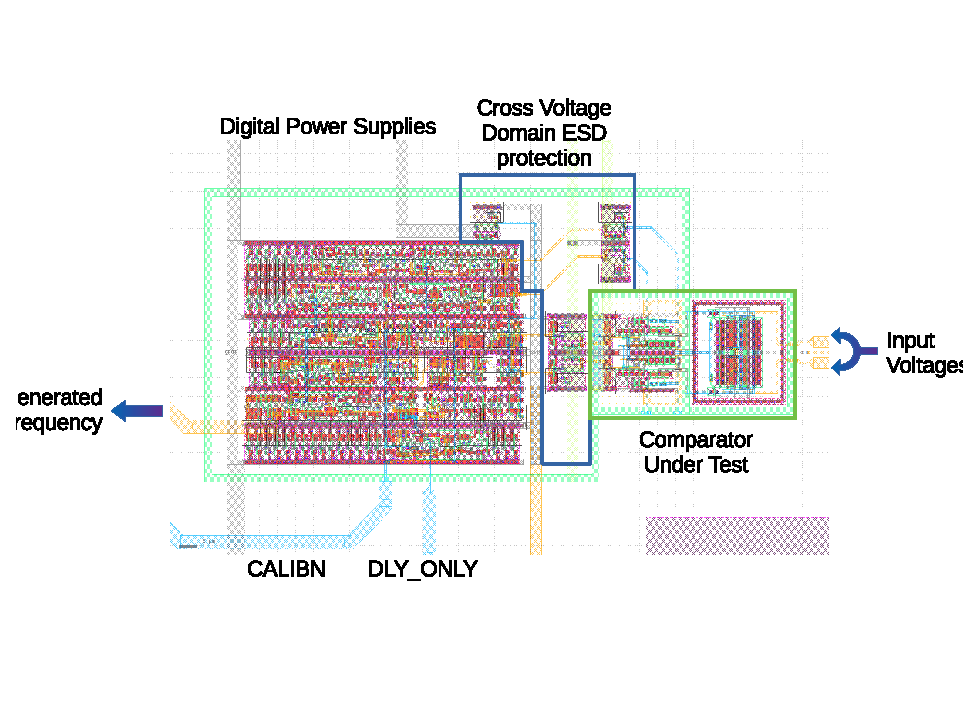
\includegraphics[width=\textwidth]{Chapter5/Figs/layout_delay_meas.eps}
        b) Layout
    \end{minipage}
    \begin{minipage}[b]{0.30\linewidth}
        \centering
        \resizebox{\textwidth}{!}{
            %% Creator: Matplotlib, PGF backend
%%
%% To include the figure in your LaTeX document, write
%%   \input{<filename>.pgf}
%%
%% Make sure the required packages are loaded in your preamble
%%   \usepackage{pgf}
%%
%% Figures using additional raster images can only be included by \input if
%% they are in the same directory as the main LaTeX file. For loading figures
%% from other directories you can use the `import` package
%%   \usepackage{import}
%% and then include the figures with
%%   \import{<path to file>}{<filename>.pgf}
%%
%% Matplotlib used the following preamble
%%   \usepackage{gensymb}
%%   \usepackage[utf8x]{inputenc}
%%   \usepackage[T1]{fontenc}
%%
\begingroup%
\makeatletter%
\begin{pgfpicture}%
\pgfpathrectangle{\pgfpointorigin}{\pgfqpoint{3.961700in}{2.962412in}}%
\pgfusepath{use as bounding box, clip}%
\begin{pgfscope}%
\pgfsetbuttcap%
\pgfsetmiterjoin%
\definecolor{currentfill}{rgb}{1.000000,1.000000,1.000000}%
\pgfsetfillcolor{currentfill}%
\pgfsetlinewidth{0.000000pt}%
\definecolor{currentstroke}{rgb}{1.000000,1.000000,1.000000}%
\pgfsetstrokecolor{currentstroke}%
\pgfsetdash{}{0pt}%
\pgfpathmoveto{\pgfqpoint{0.000000in}{0.000000in}}%
\pgfpathlineto{\pgfqpoint{3.961700in}{0.000000in}}%
\pgfpathlineto{\pgfqpoint{3.961700in}{2.962412in}}%
\pgfpathlineto{\pgfqpoint{0.000000in}{2.962412in}}%
\pgfpathclose%
\pgfusepath{fill}%
\end{pgfscope}%
\begin{pgfscope}%
\pgfsetbuttcap%
\pgfsetmiterjoin%
\definecolor{currentfill}{rgb}{1.000000,1.000000,1.000000}%
\pgfsetfillcolor{currentfill}%
\pgfsetlinewidth{0.000000pt}%
\definecolor{currentstroke}{rgb}{0.000000,0.000000,0.000000}%
\pgfsetstrokecolor{currentstroke}%
\pgfsetstrokeopacity{0.000000}%
\pgfsetdash{}{0pt}%
\pgfpathmoveto{\pgfqpoint{0.610776in}{0.489099in}}%
\pgfpathlineto{\pgfqpoint{3.757533in}{0.489099in}}%
\pgfpathlineto{\pgfqpoint{3.757533in}{2.814584in}}%
\pgfpathlineto{\pgfqpoint{0.610776in}{2.814584in}}%
\pgfpathclose%
\pgfusepath{fill}%
\end{pgfscope}%
\begin{pgfscope}%
\pgfsetbuttcap%
\pgfsetroundjoin%
\definecolor{currentfill}{rgb}{0.000000,0.000000,0.000000}%
\pgfsetfillcolor{currentfill}%
\pgfsetlinewidth{0.803000pt}%
\definecolor{currentstroke}{rgb}{0.000000,0.000000,0.000000}%
\pgfsetstrokecolor{currentstroke}%
\pgfsetdash{}{0pt}%
\pgfsys@defobject{currentmarker}{\pgfqpoint{0.000000in}{-0.048611in}}{\pgfqpoint{0.000000in}{0.000000in}}{%
\pgfpathmoveto{\pgfqpoint{0.000000in}{0.000000in}}%
\pgfpathlineto{\pgfqpoint{0.000000in}{-0.048611in}}%
\pgfusepath{stroke,fill}%
}%
\begin{pgfscope}%
\pgfsys@transformshift{0.610776in}{0.489099in}%
\pgfsys@useobject{currentmarker}{}%
\end{pgfscope}%
\end{pgfscope}%
\begin{pgfscope}%
\pgftext[x=0.610776in,y=0.391876in,,top]{\fontsize{10.000000}{12.000000}\selectfont \(\displaystyle -40\)}%
\end{pgfscope}%
\begin{pgfscope}%
\pgfsetbuttcap%
\pgfsetroundjoin%
\definecolor{currentfill}{rgb}{0.000000,0.000000,0.000000}%
\pgfsetfillcolor{currentfill}%
\pgfsetlinewidth{0.803000pt}%
\definecolor{currentstroke}{rgb}{0.000000,0.000000,0.000000}%
\pgfsetstrokecolor{currentstroke}%
\pgfsetdash{}{0pt}%
\pgfsys@defobject{currentmarker}{\pgfqpoint{0.000000in}{-0.048611in}}{\pgfqpoint{0.000000in}{0.000000in}}{%
\pgfpathmoveto{\pgfqpoint{0.000000in}{0.000000in}}%
\pgfpathlineto{\pgfqpoint{0.000000in}{-0.048611in}}%
\pgfusepath{stroke,fill}%
}%
\begin{pgfscope}%
\pgfsys@transformshift{1.196219in}{0.489099in}%
\pgfsys@useobject{currentmarker}{}%
\end{pgfscope}%
\end{pgfscope}%
\begin{pgfscope}%
\pgftext[x=1.196219in,y=0.391876in,,top]{\fontsize{10.000000}{12.000000}\selectfont \(\displaystyle 0\)}%
\end{pgfscope}%
\begin{pgfscope}%
\pgfsetbuttcap%
\pgfsetroundjoin%
\definecolor{currentfill}{rgb}{0.000000,0.000000,0.000000}%
\pgfsetfillcolor{currentfill}%
\pgfsetlinewidth{0.803000pt}%
\definecolor{currentstroke}{rgb}{0.000000,0.000000,0.000000}%
\pgfsetstrokecolor{currentstroke}%
\pgfsetdash{}{0pt}%
\pgfsys@defobject{currentmarker}{\pgfqpoint{0.000000in}{-0.048611in}}{\pgfqpoint{0.000000in}{0.000000in}}{%
\pgfpathmoveto{\pgfqpoint{0.000000in}{0.000000in}}%
\pgfpathlineto{\pgfqpoint{0.000000in}{-0.048611in}}%
\pgfusepath{stroke,fill}%
}%
\begin{pgfscope}%
\pgfsys@transformshift{1.591393in}{0.489099in}%
\pgfsys@useobject{currentmarker}{}%
\end{pgfscope}%
\end{pgfscope}%
\begin{pgfscope}%
\pgftext[x=1.591393in,y=0.391876in,,top]{\fontsize{10.000000}{12.000000}\selectfont \(\displaystyle 27\)}%
\end{pgfscope}%
\begin{pgfscope}%
\pgfsetbuttcap%
\pgfsetroundjoin%
\definecolor{currentfill}{rgb}{0.000000,0.000000,0.000000}%
\pgfsetfillcolor{currentfill}%
\pgfsetlinewidth{0.803000pt}%
\definecolor{currentstroke}{rgb}{0.000000,0.000000,0.000000}%
\pgfsetstrokecolor{currentstroke}%
\pgfsetdash{}{0pt}%
\pgfsys@defobject{currentmarker}{\pgfqpoint{0.000000in}{-0.048611in}}{\pgfqpoint{0.000000in}{0.000000in}}{%
\pgfpathmoveto{\pgfqpoint{0.000000in}{0.000000in}}%
\pgfpathlineto{\pgfqpoint{0.000000in}{-0.048611in}}%
\pgfusepath{stroke,fill}%
}%
\begin{pgfscope}%
\pgfsys@transformshift{2.440286in}{0.489099in}%
\pgfsys@useobject{currentmarker}{}%
\end{pgfscope}%
\end{pgfscope}%
\begin{pgfscope}%
\pgftext[x=2.440286in,y=0.391876in,,top]{\fontsize{10.000000}{12.000000}\selectfont \(\displaystyle 85\)}%
\end{pgfscope}%
\begin{pgfscope}%
\pgfsetbuttcap%
\pgfsetroundjoin%
\definecolor{currentfill}{rgb}{0.000000,0.000000,0.000000}%
\pgfsetfillcolor{currentfill}%
\pgfsetlinewidth{0.803000pt}%
\definecolor{currentstroke}{rgb}{0.000000,0.000000,0.000000}%
\pgfsetstrokecolor{currentstroke}%
\pgfsetdash{}{0pt}%
\pgfsys@defobject{currentmarker}{\pgfqpoint{0.000000in}{-0.048611in}}{\pgfqpoint{0.000000in}{0.000000in}}{%
\pgfpathmoveto{\pgfqpoint{0.000000in}{0.000000in}}%
\pgfpathlineto{\pgfqpoint{0.000000in}{-0.048611in}}%
\pgfusepath{stroke,fill}%
}%
\begin{pgfscope}%
\pgfsys@transformshift{3.391631in}{0.489099in}%
\pgfsys@useobject{currentmarker}{}%
\end{pgfscope}%
\end{pgfscope}%
\begin{pgfscope}%
\pgftext[x=3.391631in,y=0.391876in,,top]{\fontsize{10.000000}{12.000000}\selectfont \(\displaystyle 150\)}%
\end{pgfscope}%
\begin{pgfscope}%
\pgfsetbuttcap%
\pgfsetroundjoin%
\definecolor{currentfill}{rgb}{0.000000,0.000000,0.000000}%
\pgfsetfillcolor{currentfill}%
\pgfsetlinewidth{0.803000pt}%
\definecolor{currentstroke}{rgb}{0.000000,0.000000,0.000000}%
\pgfsetstrokecolor{currentstroke}%
\pgfsetdash{}{0pt}%
\pgfsys@defobject{currentmarker}{\pgfqpoint{0.000000in}{-0.048611in}}{\pgfqpoint{0.000000in}{0.000000in}}{%
\pgfpathmoveto{\pgfqpoint{0.000000in}{0.000000in}}%
\pgfpathlineto{\pgfqpoint{0.000000in}{-0.048611in}}%
\pgfusepath{stroke,fill}%
}%
\begin{pgfscope}%
\pgfsys@transformshift{3.757533in}{0.489099in}%
\pgfsys@useobject{currentmarker}{}%
\end{pgfscope}%
\end{pgfscope}%
\begin{pgfscope}%
\pgftext[x=3.757533in,y=0.391876in,,top]{\fontsize{10.000000}{12.000000}\selectfont \(\displaystyle 175\)}%
\end{pgfscope}%
\begin{pgfscope}%
\pgftext[x=2.184154in,y=0.213666in,,top]{\fontsize{8.000000}{9.600000}\selectfont Temperature [\(\displaystyle \degree\)C]}%
\end{pgfscope}%
\begin{pgfscope}%
\pgfsetbuttcap%
\pgfsetroundjoin%
\definecolor{currentfill}{rgb}{0.000000,0.000000,0.000000}%
\pgfsetfillcolor{currentfill}%
\pgfsetlinewidth{0.803000pt}%
\definecolor{currentstroke}{rgb}{0.000000,0.000000,0.000000}%
\pgfsetstrokecolor{currentstroke}%
\pgfsetdash{}{0pt}%
\pgfsys@defobject{currentmarker}{\pgfqpoint{-0.048611in}{0.000000in}}{\pgfqpoint{0.000000in}{0.000000in}}{%
\pgfpathmoveto{\pgfqpoint{0.000000in}{0.000000in}}%
\pgfpathlineto{\pgfqpoint{-0.048611in}{0.000000in}}%
\pgfusepath{stroke,fill}%
}%
\begin{pgfscope}%
\pgfsys@transformshift{0.610776in}{0.489099in}%
\pgfsys@useobject{currentmarker}{}%
\end{pgfscope}%
\end{pgfscope}%
\begin{pgfscope}%
\pgftext[x=0.266640in,y=0.441271in,left,base]{\fontsize{10.000000}{12.000000}\selectfont \(\displaystyle 1.25\)}%
\end{pgfscope}%
\begin{pgfscope}%
\pgfsetbuttcap%
\pgfsetroundjoin%
\definecolor{currentfill}{rgb}{0.000000,0.000000,0.000000}%
\pgfsetfillcolor{currentfill}%
\pgfsetlinewidth{0.803000pt}%
\definecolor{currentstroke}{rgb}{0.000000,0.000000,0.000000}%
\pgfsetstrokecolor{currentstroke}%
\pgfsetdash{}{0pt}%
\pgfsys@defobject{currentmarker}{\pgfqpoint{-0.048611in}{0.000000in}}{\pgfqpoint{0.000000in}{0.000000in}}{%
\pgfpathmoveto{\pgfqpoint{0.000000in}{0.000000in}}%
\pgfpathlineto{\pgfqpoint{-0.048611in}{0.000000in}}%
\pgfusepath{stroke,fill}%
}%
\begin{pgfscope}%
\pgfsys@transformshift{0.610776in}{1.070470in}%
\pgfsys@useobject{currentmarker}{}%
\end{pgfscope}%
\end{pgfscope}%
\begin{pgfscope}%
\pgftext[x=0.266640in,y=1.022642in,left,base]{\fontsize{10.000000}{12.000000}\selectfont \(\displaystyle 1.50\)}%
\end{pgfscope}%
\begin{pgfscope}%
\pgfsetbuttcap%
\pgfsetroundjoin%
\definecolor{currentfill}{rgb}{0.000000,0.000000,0.000000}%
\pgfsetfillcolor{currentfill}%
\pgfsetlinewidth{0.803000pt}%
\definecolor{currentstroke}{rgb}{0.000000,0.000000,0.000000}%
\pgfsetstrokecolor{currentstroke}%
\pgfsetdash{}{0pt}%
\pgfsys@defobject{currentmarker}{\pgfqpoint{-0.048611in}{0.000000in}}{\pgfqpoint{0.000000in}{0.000000in}}{%
\pgfpathmoveto{\pgfqpoint{0.000000in}{0.000000in}}%
\pgfpathlineto{\pgfqpoint{-0.048611in}{0.000000in}}%
\pgfusepath{stroke,fill}%
}%
\begin{pgfscope}%
\pgfsys@transformshift{0.610776in}{1.651841in}%
\pgfsys@useobject{currentmarker}{}%
\end{pgfscope}%
\end{pgfscope}%
\begin{pgfscope}%
\pgftext[x=0.266640in,y=1.604014in,left,base]{\fontsize{10.000000}{12.000000}\selectfont \(\displaystyle 1.75\)}%
\end{pgfscope}%
\begin{pgfscope}%
\pgfsetbuttcap%
\pgfsetroundjoin%
\definecolor{currentfill}{rgb}{0.000000,0.000000,0.000000}%
\pgfsetfillcolor{currentfill}%
\pgfsetlinewidth{0.803000pt}%
\definecolor{currentstroke}{rgb}{0.000000,0.000000,0.000000}%
\pgfsetstrokecolor{currentstroke}%
\pgfsetdash{}{0pt}%
\pgfsys@defobject{currentmarker}{\pgfqpoint{-0.048611in}{0.000000in}}{\pgfqpoint{0.000000in}{0.000000in}}{%
\pgfpathmoveto{\pgfqpoint{0.000000in}{0.000000in}}%
\pgfpathlineto{\pgfqpoint{-0.048611in}{0.000000in}}%
\pgfusepath{stroke,fill}%
}%
\begin{pgfscope}%
\pgfsys@transformshift{0.610776in}{2.233213in}%
\pgfsys@useobject{currentmarker}{}%
\end{pgfscope}%
\end{pgfscope}%
\begin{pgfscope}%
\pgftext[x=0.266640in,y=2.185385in,left,base]{\fontsize{10.000000}{12.000000}\selectfont \(\displaystyle 2.00\)}%
\end{pgfscope}%
\begin{pgfscope}%
\pgfsetbuttcap%
\pgfsetroundjoin%
\definecolor{currentfill}{rgb}{0.000000,0.000000,0.000000}%
\pgfsetfillcolor{currentfill}%
\pgfsetlinewidth{0.803000pt}%
\definecolor{currentstroke}{rgb}{0.000000,0.000000,0.000000}%
\pgfsetstrokecolor{currentstroke}%
\pgfsetdash{}{0pt}%
\pgfsys@defobject{currentmarker}{\pgfqpoint{-0.048611in}{0.000000in}}{\pgfqpoint{0.000000in}{0.000000in}}{%
\pgfpathmoveto{\pgfqpoint{0.000000in}{0.000000in}}%
\pgfpathlineto{\pgfqpoint{-0.048611in}{0.000000in}}%
\pgfusepath{stroke,fill}%
}%
\begin{pgfscope}%
\pgfsys@transformshift{0.610776in}{2.814584in}%
\pgfsys@useobject{currentmarker}{}%
\end{pgfscope}%
\end{pgfscope}%
\begin{pgfscope}%
\pgftext[x=0.266640in,y=2.766756in,left,base]{\fontsize{10.000000}{12.000000}\selectfont \(\displaystyle 2.25\)}%
\end{pgfscope}%
\begin{pgfscope}%
\pgftext[x=0.211084in,y=1.651841in,,bottom,rotate=90.000000]{\fontsize{8.000000}{9.600000}\selectfont D'elai [ns]}%
\end{pgfscope}%
\begin{pgfscope}%
\pgfpathrectangle{\pgfqpoint{0.610776in}{0.489099in}}{\pgfqpoint{3.146757in}{2.325486in}} %
\pgfusepath{clip}%
\pgfsetrectcap%
\pgfsetroundjoin%
\pgfsetlinewidth{2.007500pt}%
\definecolor{currentstroke}{rgb}{1.000000,0.000000,0.000000}%
\pgfsetstrokecolor{currentstroke}%
\pgfsetdash{}{0pt}%
\pgfpathmoveto{\pgfqpoint{0.610776in}{0.554069in}}%
\pgfpathlineto{\pgfqpoint{0.830317in}{0.684222in}}%
\pgfpathlineto{\pgfqpoint{1.196219in}{0.895756in}}%
\pgfpathlineto{\pgfqpoint{1.562121in}{1.101127in}}%
\pgfpathlineto{\pgfqpoint{1.591393in}{1.114632in}}%
\pgfpathlineto{\pgfqpoint{2.103656in}{1.389943in}}%
\pgfpathlineto{\pgfqpoint{2.440286in}{1.557671in}}%
\pgfpathlineto{\pgfqpoint{2.659827in}{1.713567in}}%
\pgfpathlineto{\pgfqpoint{3.025729in}{1.907846in}}%
\pgfpathlineto{\pgfqpoint{3.391631in}{2.113404in}}%
\pgfpathlineto{\pgfqpoint{3.757533in}{2.360913in}}%
\pgfusepath{stroke}%
\end{pgfscope}%
\begin{pgfscope}%
\pgfpathrectangle{\pgfqpoint{0.610776in}{0.489099in}}{\pgfqpoint{3.146757in}{2.325486in}} %
\pgfusepath{clip}%
\pgfsetbuttcap%
\pgfsetroundjoin%
\definecolor{currentfill}{rgb}{0.000000,0.000000,0.000000}%
\pgfsetfillcolor{currentfill}%
\pgfsetlinewidth{1.003750pt}%
\definecolor{currentstroke}{rgb}{0.000000,0.000000,0.000000}%
\pgfsetstrokecolor{currentstroke}%
\pgfsetdash{}{0pt}%
\pgfsys@defobject{currentmarker}{\pgfqpoint{-0.020833in}{-0.020833in}}{\pgfqpoint{0.020833in}{0.020833in}}{%
\pgfpathmoveto{\pgfqpoint{0.000000in}{-0.020833in}}%
\pgfpathcurveto{\pgfqpoint{0.005525in}{-0.020833in}}{\pgfqpoint{0.010825in}{-0.018638in}}{\pgfqpoint{0.014731in}{-0.014731in}}%
\pgfpathcurveto{\pgfqpoint{0.018638in}{-0.010825in}}{\pgfqpoint{0.020833in}{-0.005525in}}{\pgfqpoint{0.020833in}{0.000000in}}%
\pgfpathcurveto{\pgfqpoint{0.020833in}{0.005525in}}{\pgfqpoint{0.018638in}{0.010825in}}{\pgfqpoint{0.014731in}{0.014731in}}%
\pgfpathcurveto{\pgfqpoint{0.010825in}{0.018638in}}{\pgfqpoint{0.005525in}{0.020833in}}{\pgfqpoint{0.000000in}{0.020833in}}%
\pgfpathcurveto{\pgfqpoint{-0.005525in}{0.020833in}}{\pgfqpoint{-0.010825in}{0.018638in}}{\pgfqpoint{-0.014731in}{0.014731in}}%
\pgfpathcurveto{\pgfqpoint{-0.018638in}{0.010825in}}{\pgfqpoint{-0.020833in}{0.005525in}}{\pgfqpoint{-0.020833in}{0.000000in}}%
\pgfpathcurveto{\pgfqpoint{-0.020833in}{-0.005525in}}{\pgfqpoint{-0.018638in}{-0.010825in}}{\pgfqpoint{-0.014731in}{-0.014731in}}%
\pgfpathcurveto{\pgfqpoint{-0.010825in}{-0.018638in}}{\pgfqpoint{-0.005525in}{-0.020833in}}{\pgfqpoint{0.000000in}{-0.020833in}}%
\pgfpathclose%
\pgfusepath{stroke,fill}%
}%
\begin{pgfscope}%
\pgfsys@transformshift{0.610776in}{0.520228in}%
\pgfsys@useobject{currentmarker}{}%
\end{pgfscope}%
\begin{pgfscope}%
\pgfsys@transformshift{0.830317in}{0.632491in}%
\pgfsys@useobject{currentmarker}{}%
\end{pgfscope}%
\begin{pgfscope}%
\pgfsys@transformshift{1.196219in}{0.810982in}%
\pgfsys@useobject{currentmarker}{}%
\end{pgfscope}%
\begin{pgfscope}%
\pgfsys@transformshift{1.562121in}{0.966724in}%
\pgfsys@useobject{currentmarker}{}%
\end{pgfscope}%
\begin{pgfscope}%
\pgfsys@transformshift{1.576757in}{0.978761in}%
\pgfsys@useobject{currentmarker}{}%
\end{pgfscope}%
\begin{pgfscope}%
\pgfsys@transformshift{1.591393in}{0.977679in}%
\pgfsys@useobject{currentmarker}{}%
\end{pgfscope}%
\begin{pgfscope}%
\pgfsys@transformshift{1.598711in}{0.993676in}%
\pgfsys@useobject{currentmarker}{}%
\end{pgfscope}%
\begin{pgfscope}%
\pgfsys@transformshift{1.928023in}{1.192563in}%
\pgfsys@useobject{currentmarker}{}%
\end{pgfscope}%
\begin{pgfscope}%
\pgfsys@transformshift{2.367105in}{1.444402in}%
\pgfsys@useobject{currentmarker}{}%
\end{pgfscope}%
\begin{pgfscope}%
\pgfsys@transformshift{2.659827in}{1.644734in}%
\pgfsys@useobject{currentmarker}{}%
\end{pgfscope}%
\begin{pgfscope}%
\pgfsys@transformshift{3.025729in}{1.881437in}%
\pgfsys@useobject{currentmarker}{}%
\end{pgfscope}%
\begin{pgfscope}%
\pgfsys@transformshift{3.245270in}{2.028786in}%
\pgfsys@useobject{currentmarker}{}%
\end{pgfscope}%
\begin{pgfscope}%
\pgfsys@transformshift{3.391631in}{2.135870in}%
\pgfsys@useobject{currentmarker}{}%
\end{pgfscope}%
\begin{pgfscope}%
\pgfsys@transformshift{3.537991in}{2.242192in}%
\pgfsys@useobject{currentmarker}{}%
\end{pgfscope}%
\begin{pgfscope}%
\pgfsys@transformshift{3.684352in}{2.348776in}%
\pgfsys@useobject{currentmarker}{}%
\end{pgfscope}%
\begin{pgfscope}%
\pgfsys@transformshift{3.757533in}{2.398322in}%
\pgfsys@useobject{currentmarker}{}%
\end{pgfscope}%
\end{pgfscope}%
\begin{pgfscope}%
\pgfpathrectangle{\pgfqpoint{0.610776in}{0.489099in}}{\pgfqpoint{3.146757in}{2.325486in}} %
\pgfusepath{clip}%
\pgfsetbuttcap%
\pgfsetroundjoin%
\definecolor{currentfill}{rgb}{0.000000,0.500000,0.000000}%
\pgfsetfillcolor{currentfill}%
\pgfsetlinewidth{1.003750pt}%
\definecolor{currentstroke}{rgb}{0.000000,0.500000,0.000000}%
\pgfsetstrokecolor{currentstroke}%
\pgfsetdash{}{0pt}%
\pgfsys@defobject{currentmarker}{\pgfqpoint{-0.020833in}{-0.020833in}}{\pgfqpoint{0.020833in}{0.020833in}}{%
\pgfpathmoveto{\pgfqpoint{0.000000in}{-0.020833in}}%
\pgfpathcurveto{\pgfqpoint{0.005525in}{-0.020833in}}{\pgfqpoint{0.010825in}{-0.018638in}}{\pgfqpoint{0.014731in}{-0.014731in}}%
\pgfpathcurveto{\pgfqpoint{0.018638in}{-0.010825in}}{\pgfqpoint{0.020833in}{-0.005525in}}{\pgfqpoint{0.020833in}{0.000000in}}%
\pgfpathcurveto{\pgfqpoint{0.020833in}{0.005525in}}{\pgfqpoint{0.018638in}{0.010825in}}{\pgfqpoint{0.014731in}{0.014731in}}%
\pgfpathcurveto{\pgfqpoint{0.010825in}{0.018638in}}{\pgfqpoint{0.005525in}{0.020833in}}{\pgfqpoint{0.000000in}{0.020833in}}%
\pgfpathcurveto{\pgfqpoint{-0.005525in}{0.020833in}}{\pgfqpoint{-0.010825in}{0.018638in}}{\pgfqpoint{-0.014731in}{0.014731in}}%
\pgfpathcurveto{\pgfqpoint{-0.018638in}{0.010825in}}{\pgfqpoint{-0.020833in}{0.005525in}}{\pgfqpoint{-0.020833in}{0.000000in}}%
\pgfpathcurveto{\pgfqpoint{-0.020833in}{-0.005525in}}{\pgfqpoint{-0.018638in}{-0.010825in}}{\pgfqpoint{-0.014731in}{-0.014731in}}%
\pgfpathcurveto{\pgfqpoint{-0.010825in}{-0.018638in}}{\pgfqpoint{-0.005525in}{-0.020833in}}{\pgfqpoint{0.000000in}{-0.020833in}}%
\pgfpathclose%
\pgfusepath{stroke,fill}%
}%
\begin{pgfscope}%
\pgfsys@transformshift{0.610776in}{0.631593in}%
\pgfsys@useobject{currentmarker}{}%
\end{pgfscope}%
\begin{pgfscope}%
\pgfsys@transformshift{0.757137in}{0.713028in}%
\pgfsys@useobject{currentmarker}{}%
\end{pgfscope}%
\begin{pgfscope}%
\pgfsys@transformshift{0.830317in}{0.768294in}%
\pgfsys@useobject{currentmarker}{}%
\end{pgfscope}%
\begin{pgfscope}%
\pgfsys@transformshift{0.903498in}{0.802436in}%
\pgfsys@useobject{currentmarker}{}%
\end{pgfscope}%
\begin{pgfscope}%
\pgfsys@transformshift{1.049858in}{0.795605in}%
\pgfsys@useobject{currentmarker}{}%
\end{pgfscope}%
\begin{pgfscope}%
\pgfsys@transformshift{1.196219in}{0.870740in}%
\pgfsys@useobject{currentmarker}{}%
\end{pgfscope}%
\begin{pgfscope}%
\pgfsys@transformshift{1.342580in}{0.952263in}%
\pgfsys@useobject{currentmarker}{}%
\end{pgfscope}%
\begin{pgfscope}%
\pgfsys@transformshift{1.488941in}{1.054454in}%
\pgfsys@useobject{currentmarker}{}%
\end{pgfscope}%
\begin{pgfscope}%
\pgfsys@transformshift{1.562121in}{1.080085in}%
\pgfsys@useobject{currentmarker}{}%
\end{pgfscope}%
\begin{pgfscope}%
\pgfsys@transformshift{1.591393in}{1.155207in}%
\pgfsys@useobject{currentmarker}{}%
\end{pgfscope}%
\begin{pgfscope}%
\pgfsys@transformshift{1.598711in}{0.975990in}%
\pgfsys@useobject{currentmarker}{}%
\end{pgfscope}%
\begin{pgfscope}%
\pgfsys@transformshift{1.635301in}{1.133599in}%
\pgfsys@useobject{currentmarker}{}%
\end{pgfscope}%
\begin{pgfscope}%
\pgfsys@transformshift{1.781662in}{1.222368in}%
\pgfsys@useobject{currentmarker}{}%
\end{pgfscope}%
\begin{pgfscope}%
\pgfsys@transformshift{1.928023in}{1.303555in}%
\pgfsys@useobject{currentmarker}{}%
\end{pgfscope}%
\begin{pgfscope}%
\pgfsys@transformshift{2.074384in}{1.409265in}%
\pgfsys@useobject{currentmarker}{}%
\end{pgfscope}%
\begin{pgfscope}%
\pgfsys@transformshift{2.220745in}{1.488263in}%
\pgfsys@useobject{currentmarker}{}%
\end{pgfscope}%
\begin{pgfscope}%
\pgfsys@transformshift{2.367105in}{1.590297in}%
\pgfsys@useobject{currentmarker}{}%
\end{pgfscope}%
\begin{pgfscope}%
\pgfsys@transformshift{2.513466in}{1.673493in}%
\pgfsys@useobject{currentmarker}{}%
\end{pgfscope}%
\begin{pgfscope}%
\pgfsys@transformshift{2.659827in}{1.778264in}%
\pgfsys@useobject{currentmarker}{}%
\end{pgfscope}%
\begin{pgfscope}%
\pgfsys@transformshift{2.806188in}{1.770412in}%
\pgfsys@useobject{currentmarker}{}%
\end{pgfscope}%
\begin{pgfscope}%
\pgfsys@transformshift{2.952548in}{1.864897in}%
\pgfsys@useobject{currentmarker}{}%
\end{pgfscope}%
\begin{pgfscope}%
\pgfsys@transformshift{3.025729in}{1.915040in}%
\pgfsys@useobject{currentmarker}{}%
\end{pgfscope}%
\begin{pgfscope}%
\pgfsys@transformshift{3.098909in}{1.964185in}%
\pgfsys@useobject{currentmarker}{}%
\end{pgfscope}%
\begin{pgfscope}%
\pgfsys@transformshift{3.245270in}{2.070006in}%
\pgfsys@useobject{currentmarker}{}%
\end{pgfscope}%
\begin{pgfscope}%
\pgfsys@transformshift{3.391631in}{2.172868in}%
\pgfsys@useobject{currentmarker}{}%
\end{pgfscope}%
\begin{pgfscope}%
\pgfsys@transformshift{3.537991in}{2.275951in}%
\pgfsys@useobject{currentmarker}{}%
\end{pgfscope}%
\begin{pgfscope}%
\pgfsys@transformshift{3.684352in}{2.388773in}%
\pgfsys@useobject{currentmarker}{}%
\end{pgfscope}%
\begin{pgfscope}%
\pgfsys@transformshift{3.757533in}{2.458560in}%
\pgfsys@useobject{currentmarker}{}%
\end{pgfscope}%
\end{pgfscope}%
\begin{pgfscope}%
\pgfpathrectangle{\pgfqpoint{0.610776in}{0.489099in}}{\pgfqpoint{3.146757in}{2.325486in}} %
\pgfusepath{clip}%
\pgfsetbuttcap%
\pgfsetroundjoin%
\definecolor{currentfill}{rgb}{0.000000,0.000000,1.000000}%
\pgfsetfillcolor{currentfill}%
\pgfsetlinewidth{1.003750pt}%
\definecolor{currentstroke}{rgb}{0.000000,0.000000,1.000000}%
\pgfsetstrokecolor{currentstroke}%
\pgfsetdash{}{0pt}%
\pgfsys@defobject{currentmarker}{\pgfqpoint{-0.020833in}{-0.020833in}}{\pgfqpoint{0.020833in}{0.020833in}}{%
\pgfpathmoveto{\pgfqpoint{0.000000in}{-0.020833in}}%
\pgfpathcurveto{\pgfqpoint{0.005525in}{-0.020833in}}{\pgfqpoint{0.010825in}{-0.018638in}}{\pgfqpoint{0.014731in}{-0.014731in}}%
\pgfpathcurveto{\pgfqpoint{0.018638in}{-0.010825in}}{\pgfqpoint{0.020833in}{-0.005525in}}{\pgfqpoint{0.020833in}{0.000000in}}%
\pgfpathcurveto{\pgfqpoint{0.020833in}{0.005525in}}{\pgfqpoint{0.018638in}{0.010825in}}{\pgfqpoint{0.014731in}{0.014731in}}%
\pgfpathcurveto{\pgfqpoint{0.010825in}{0.018638in}}{\pgfqpoint{0.005525in}{0.020833in}}{\pgfqpoint{0.000000in}{0.020833in}}%
\pgfpathcurveto{\pgfqpoint{-0.005525in}{0.020833in}}{\pgfqpoint{-0.010825in}{0.018638in}}{\pgfqpoint{-0.014731in}{0.014731in}}%
\pgfpathcurveto{\pgfqpoint{-0.018638in}{0.010825in}}{\pgfqpoint{-0.020833in}{0.005525in}}{\pgfqpoint{-0.020833in}{0.000000in}}%
\pgfpathcurveto{\pgfqpoint{-0.020833in}{-0.005525in}}{\pgfqpoint{-0.018638in}{-0.010825in}}{\pgfqpoint{-0.014731in}{-0.014731in}}%
\pgfpathcurveto{\pgfqpoint{-0.010825in}{-0.018638in}}{\pgfqpoint{-0.005525in}{-0.020833in}}{\pgfqpoint{0.000000in}{-0.020833in}}%
\pgfpathclose%
\pgfusepath{stroke,fill}%
}%
\begin{pgfscope}%
\pgfsys@transformshift{0.610776in}{0.587210in}%
\pgfsys@useobject{currentmarker}{}%
\end{pgfscope}%
\begin{pgfscope}%
\pgfsys@transformshift{0.830317in}{0.732885in}%
\pgfsys@useobject{currentmarker}{}%
\end{pgfscope}%
\begin{pgfscope}%
\pgfsys@transformshift{1.196219in}{0.927831in}%
\pgfsys@useobject{currentmarker}{}%
\end{pgfscope}%
\begin{pgfscope}%
\pgfsys@transformshift{1.562121in}{1.080683in}%
\pgfsys@useobject{currentmarker}{}%
\end{pgfscope}%
\begin{pgfscope}%
\pgfsys@transformshift{1.591393in}{1.110380in}%
\pgfsys@useobject{currentmarker}{}%
\end{pgfscope}%
\begin{pgfscope}%
\pgfsys@transformshift{1.598711in}{1.122384in}%
\pgfsys@useobject{currentmarker}{}%
\end{pgfscope}%
\begin{pgfscope}%
\pgfsys@transformshift{1.928023in}{1.330417in}%
\pgfsys@useobject{currentmarker}{}%
\end{pgfscope}%
\begin{pgfscope}%
\pgfsys@transformshift{2.367105in}{1.573417in}%
\pgfsys@useobject{currentmarker}{}%
\end{pgfscope}%
\begin{pgfscope}%
\pgfsys@transformshift{2.659827in}{1.795402in}%
\pgfsys@useobject{currentmarker}{}%
\end{pgfscope}%
\begin{pgfscope}%
\pgfsys@transformshift{3.025729in}{1.893013in}%
\pgfsys@useobject{currentmarker}{}%
\end{pgfscope}%
\begin{pgfscope}%
\pgfsys@transformshift{3.245270in}{2.068597in}%
\pgfsys@useobject{currentmarker}{}%
\end{pgfscope}%
\begin{pgfscope}%
\pgfsys@transformshift{3.391631in}{2.160189in}%
\pgfsys@useobject{currentmarker}{}%
\end{pgfscope}%
\begin{pgfscope}%
\pgfsys@transformshift{3.537991in}{2.294410in}%
\pgfsys@useobject{currentmarker}{}%
\end{pgfscope}%
\begin{pgfscope}%
\pgfsys@transformshift{3.684352in}{2.394205in}%
\pgfsys@useobject{currentmarker}{}%
\end{pgfscope}%
\begin{pgfscope}%
\pgfsys@transformshift{3.757533in}{2.532729in}%
\pgfsys@useobject{currentmarker}{}%
\end{pgfscope}%
\end{pgfscope}%
\begin{pgfscope}%
\pgfsetrectcap%
\pgfsetmiterjoin%
\pgfsetlinewidth{0.803000pt}%
\definecolor{currentstroke}{rgb}{0.000000,0.000000,0.000000}%
\pgfsetstrokecolor{currentstroke}%
\pgfsetdash{}{0pt}%
\pgfpathmoveto{\pgfqpoint{0.610776in}{0.489099in}}%
\pgfpathlineto{\pgfqpoint{0.610776in}{2.814584in}}%
\pgfusepath{stroke}%
\end{pgfscope}%
\begin{pgfscope}%
\pgfsetrectcap%
\pgfsetmiterjoin%
\pgfsetlinewidth{0.803000pt}%
\definecolor{currentstroke}{rgb}{0.000000,0.000000,0.000000}%
\pgfsetstrokecolor{currentstroke}%
\pgfsetdash{}{0pt}%
\pgfpathmoveto{\pgfqpoint{3.757533in}{0.489099in}}%
\pgfpathlineto{\pgfqpoint{3.757533in}{2.814584in}}%
\pgfusepath{stroke}%
\end{pgfscope}%
\begin{pgfscope}%
\pgfsetrectcap%
\pgfsetmiterjoin%
\pgfsetlinewidth{0.803000pt}%
\definecolor{currentstroke}{rgb}{0.000000,0.000000,0.000000}%
\pgfsetstrokecolor{currentstroke}%
\pgfsetdash{}{0pt}%
\pgfpathmoveto{\pgfqpoint{0.610776in}{0.489099in}}%
\pgfpathlineto{\pgfqpoint{3.757533in}{0.489099in}}%
\pgfusepath{stroke}%
\end{pgfscope}%
\begin{pgfscope}%
\pgfsetrectcap%
\pgfsetmiterjoin%
\pgfsetlinewidth{0.803000pt}%
\definecolor{currentstroke}{rgb}{0.000000,0.000000,0.000000}%
\pgfsetstrokecolor{currentstroke}%
\pgfsetdash{}{0pt}%
\pgfpathmoveto{\pgfqpoint{0.610776in}{2.814584in}}%
\pgfpathlineto{\pgfqpoint{3.757533in}{2.814584in}}%
\pgfusepath{stroke}%
\end{pgfscope}%
\begin{pgfscope}%
\pgfsetbuttcap%
\pgfsetmiterjoin%
\definecolor{currentfill}{rgb}{1.000000,1.000000,1.000000}%
\pgfsetfillcolor{currentfill}%
\pgfsetfillopacity{0.800000}%
\pgfsetlinewidth{1.003750pt}%
\definecolor{currentstroke}{rgb}{0.800000,0.800000,0.800000}%
\pgfsetstrokecolor{currentstroke}%
\pgfsetstrokeopacity{0.800000}%
\pgfsetdash{}{0pt}%
\pgfpathmoveto{\pgfqpoint{0.707998in}{1.928808in}}%
\pgfpathlineto{\pgfqpoint{2.392495in}{1.928808in}}%
\pgfpathquadraticcurveto{\pgfqpoint{2.420273in}{1.928808in}}{\pgfqpoint{2.420273in}{1.956586in}}%
\pgfpathlineto{\pgfqpoint{2.420273in}{2.717362in}}%
\pgfpathquadraticcurveto{\pgfqpoint{2.420273in}{2.745140in}}{\pgfqpoint{2.392495in}{2.745140in}}%
\pgfpathlineto{\pgfqpoint{0.707998in}{2.745140in}}%
\pgfpathquadraticcurveto{\pgfqpoint{0.680221in}{2.745140in}}{\pgfqpoint{0.680221in}{2.717362in}}%
\pgfpathlineto{\pgfqpoint{0.680221in}{1.956586in}}%
\pgfpathquadraticcurveto{\pgfqpoint{0.680221in}{1.928808in}}{\pgfqpoint{0.707998in}{1.928808in}}%
\pgfpathclose%
\pgfusepath{stroke,fill}%
\end{pgfscope}%
\begin{pgfscope}%
\pgfsetrectcap%
\pgfsetroundjoin%
\pgfsetlinewidth{2.007500pt}%
\definecolor{currentstroke}{rgb}{1.000000,0.000000,0.000000}%
\pgfsetstrokecolor{currentstroke}%
\pgfsetdash{}{0pt}%
\pgfpathmoveto{\pgfqpoint{0.735776in}{2.640973in}}%
\pgfpathlineto{\pgfqpoint{1.013554in}{2.640973in}}%
\pgfusepath{stroke}%
\end{pgfscope}%
\begin{pgfscope}%
\pgftext[x=1.124665in,y=2.592362in,left,base]{\fontsize{10.000000}{12.000000}\selectfont Post-Layout}%
\end{pgfscope}%
\begin{pgfscope}%
\pgfsetbuttcap%
\pgfsetroundjoin%
\definecolor{currentfill}{rgb}{0.000000,0.000000,0.000000}%
\pgfsetfillcolor{currentfill}%
\pgfsetlinewidth{1.003750pt}%
\definecolor{currentstroke}{rgb}{0.000000,0.000000,0.000000}%
\pgfsetstrokecolor{currentstroke}%
\pgfsetdash{}{0pt}%
\pgfsys@defobject{currentmarker}{\pgfqpoint{-0.020833in}{-0.020833in}}{\pgfqpoint{0.020833in}{0.020833in}}{%
\pgfpathmoveto{\pgfqpoint{0.000000in}{-0.020833in}}%
\pgfpathcurveto{\pgfqpoint{0.005525in}{-0.020833in}}{\pgfqpoint{0.010825in}{-0.018638in}}{\pgfqpoint{0.014731in}{-0.014731in}}%
\pgfpathcurveto{\pgfqpoint{0.018638in}{-0.010825in}}{\pgfqpoint{0.020833in}{-0.005525in}}{\pgfqpoint{0.020833in}{0.000000in}}%
\pgfpathcurveto{\pgfqpoint{0.020833in}{0.005525in}}{\pgfqpoint{0.018638in}{0.010825in}}{\pgfqpoint{0.014731in}{0.014731in}}%
\pgfpathcurveto{\pgfqpoint{0.010825in}{0.018638in}}{\pgfqpoint{0.005525in}{0.020833in}}{\pgfqpoint{0.000000in}{0.020833in}}%
\pgfpathcurveto{\pgfqpoint{-0.005525in}{0.020833in}}{\pgfqpoint{-0.010825in}{0.018638in}}{\pgfqpoint{-0.014731in}{0.014731in}}%
\pgfpathcurveto{\pgfqpoint{-0.018638in}{0.010825in}}{\pgfqpoint{-0.020833in}{0.005525in}}{\pgfqpoint{-0.020833in}{0.000000in}}%
\pgfpathcurveto{\pgfqpoint{-0.020833in}{-0.005525in}}{\pgfqpoint{-0.018638in}{-0.010825in}}{\pgfqpoint{-0.014731in}{-0.014731in}}%
\pgfpathcurveto{\pgfqpoint{-0.010825in}{-0.018638in}}{\pgfqpoint{-0.005525in}{-0.020833in}}{\pgfqpoint{0.000000in}{-0.020833in}}%
\pgfpathclose%
\pgfusepath{stroke,fill}%
}%
\begin{pgfscope}%
\pgfsys@transformshift{0.874665in}{2.447307in}%
\pgfsys@useobject{currentmarker}{}%
\end{pgfscope}%
\end{pgfscope}%
\begin{pgfscope}%
\pgftext[x=1.124665in,y=2.398696in,left,base]{\fontsize{10.000000}{12.000000}\selectfont Measures DOE03-13}%
\end{pgfscope}%
\begin{pgfscope}%
\pgfsetbuttcap%
\pgfsetroundjoin%
\definecolor{currentfill}{rgb}{0.000000,0.500000,0.000000}%
\pgfsetfillcolor{currentfill}%
\pgfsetlinewidth{1.003750pt}%
\definecolor{currentstroke}{rgb}{0.000000,0.500000,0.000000}%
\pgfsetstrokecolor{currentstroke}%
\pgfsetdash{}{0pt}%
\pgfsys@defobject{currentmarker}{\pgfqpoint{-0.020833in}{-0.020833in}}{\pgfqpoint{0.020833in}{0.020833in}}{%
\pgfpathmoveto{\pgfqpoint{0.000000in}{-0.020833in}}%
\pgfpathcurveto{\pgfqpoint{0.005525in}{-0.020833in}}{\pgfqpoint{0.010825in}{-0.018638in}}{\pgfqpoint{0.014731in}{-0.014731in}}%
\pgfpathcurveto{\pgfqpoint{0.018638in}{-0.010825in}}{\pgfqpoint{0.020833in}{-0.005525in}}{\pgfqpoint{0.020833in}{0.000000in}}%
\pgfpathcurveto{\pgfqpoint{0.020833in}{0.005525in}}{\pgfqpoint{0.018638in}{0.010825in}}{\pgfqpoint{0.014731in}{0.014731in}}%
\pgfpathcurveto{\pgfqpoint{0.010825in}{0.018638in}}{\pgfqpoint{0.005525in}{0.020833in}}{\pgfqpoint{0.000000in}{0.020833in}}%
\pgfpathcurveto{\pgfqpoint{-0.005525in}{0.020833in}}{\pgfqpoint{-0.010825in}{0.018638in}}{\pgfqpoint{-0.014731in}{0.014731in}}%
\pgfpathcurveto{\pgfqpoint{-0.018638in}{0.010825in}}{\pgfqpoint{-0.020833in}{0.005525in}}{\pgfqpoint{-0.020833in}{0.000000in}}%
\pgfpathcurveto{\pgfqpoint{-0.020833in}{-0.005525in}}{\pgfqpoint{-0.018638in}{-0.010825in}}{\pgfqpoint{-0.014731in}{-0.014731in}}%
\pgfpathcurveto{\pgfqpoint{-0.010825in}{-0.018638in}}{\pgfqpoint{-0.005525in}{-0.020833in}}{\pgfqpoint{0.000000in}{-0.020833in}}%
\pgfpathclose%
\pgfusepath{stroke,fill}%
}%
\begin{pgfscope}%
\pgfsys@transformshift{0.874665in}{2.253641in}%
\pgfsys@useobject{currentmarker}{}%
\end{pgfscope}%
\end{pgfscope}%
\begin{pgfscope}%
\pgftext[x=1.124665in,y=2.205029in,left,base]{\fontsize{10.000000}{12.000000}\selectfont Measures DOE03-15}%
\end{pgfscope}%
\begin{pgfscope}%
\pgfsetbuttcap%
\pgfsetroundjoin%
\definecolor{currentfill}{rgb}{0.000000,0.000000,1.000000}%
\pgfsetfillcolor{currentfill}%
\pgfsetlinewidth{1.003750pt}%
\definecolor{currentstroke}{rgb}{0.000000,0.000000,1.000000}%
\pgfsetstrokecolor{currentstroke}%
\pgfsetdash{}{0pt}%
\pgfsys@defobject{currentmarker}{\pgfqpoint{-0.020833in}{-0.020833in}}{\pgfqpoint{0.020833in}{0.020833in}}{%
\pgfpathmoveto{\pgfqpoint{0.000000in}{-0.020833in}}%
\pgfpathcurveto{\pgfqpoint{0.005525in}{-0.020833in}}{\pgfqpoint{0.010825in}{-0.018638in}}{\pgfqpoint{0.014731in}{-0.014731in}}%
\pgfpathcurveto{\pgfqpoint{0.018638in}{-0.010825in}}{\pgfqpoint{0.020833in}{-0.005525in}}{\pgfqpoint{0.020833in}{0.000000in}}%
\pgfpathcurveto{\pgfqpoint{0.020833in}{0.005525in}}{\pgfqpoint{0.018638in}{0.010825in}}{\pgfqpoint{0.014731in}{0.014731in}}%
\pgfpathcurveto{\pgfqpoint{0.010825in}{0.018638in}}{\pgfqpoint{0.005525in}{0.020833in}}{\pgfqpoint{0.000000in}{0.020833in}}%
\pgfpathcurveto{\pgfqpoint{-0.005525in}{0.020833in}}{\pgfqpoint{-0.010825in}{0.018638in}}{\pgfqpoint{-0.014731in}{0.014731in}}%
\pgfpathcurveto{\pgfqpoint{-0.018638in}{0.010825in}}{\pgfqpoint{-0.020833in}{0.005525in}}{\pgfqpoint{-0.020833in}{0.000000in}}%
\pgfpathcurveto{\pgfqpoint{-0.020833in}{-0.005525in}}{\pgfqpoint{-0.018638in}{-0.010825in}}{\pgfqpoint{-0.014731in}{-0.014731in}}%
\pgfpathcurveto{\pgfqpoint{-0.010825in}{-0.018638in}}{\pgfqpoint{-0.005525in}{-0.020833in}}{\pgfqpoint{0.000000in}{-0.020833in}}%
\pgfpathclose%
\pgfusepath{stroke,fill}%
}%
\begin{pgfscope}%
\pgfsys@transformshift{0.874665in}{2.059974in}%
\pgfsys@useobject{currentmarker}{}%
\end{pgfscope}%
\end{pgfscope}%
\begin{pgfscope}%
\pgftext[x=1.124665in,y=2.011363in,left,base]{\fontsize{10.000000}{12.000000}\selectfont Measures DOE03-19}%
\end{pgfscope}%
\end{pgfpicture}%
\makeatother%
\endgroup%

        }
        c) Mesures
    \end{minipage}
    \caption[]{Auto-oscillateur asynchrone pour la mesure différentielle du délai avec une résolution de 60 ps}
	\label{fig:meas_circ_schem-fr}
\end{center}

Au final, les résultats préliminaires sont encourageants sur les capacités de l'architecture hybride proposée en vue d'une haute résolution à une vitesse d'échantillonnage modérée. Le convertisseur réalisé dans une technologie SOI CMOS 180 nm, a une sensibilité vis-à-vis de la température moindre en comparaison de convertisseurs analogique-numérique en haute température publiés puisque ceux-ci subissent une chute de 2-bits sur la même plage de températures~\cite{Ericson2004}. La résolution espérée serait de 11,2 bits et 13,2 bits pour respectivement un sur-échantillonnage de 5 et 6 coups d'horloge. Cela correspond à un facteur de mérite de Walden valant 124 fJ/conversion et un facteur de mérite de Schreier valant 159. Ceci place la nouvelle architecture réalisée dans la frange moyenne des convertisseurs analogique-numérique selon le critère de Walden, et le critère de Schreier tel que représenté dans la \figurename~\ref{fig:fom-fr}.

\begin{center}
    \centering
    \begin{minipage}[b]{0.49\linewidth}
        \centering
        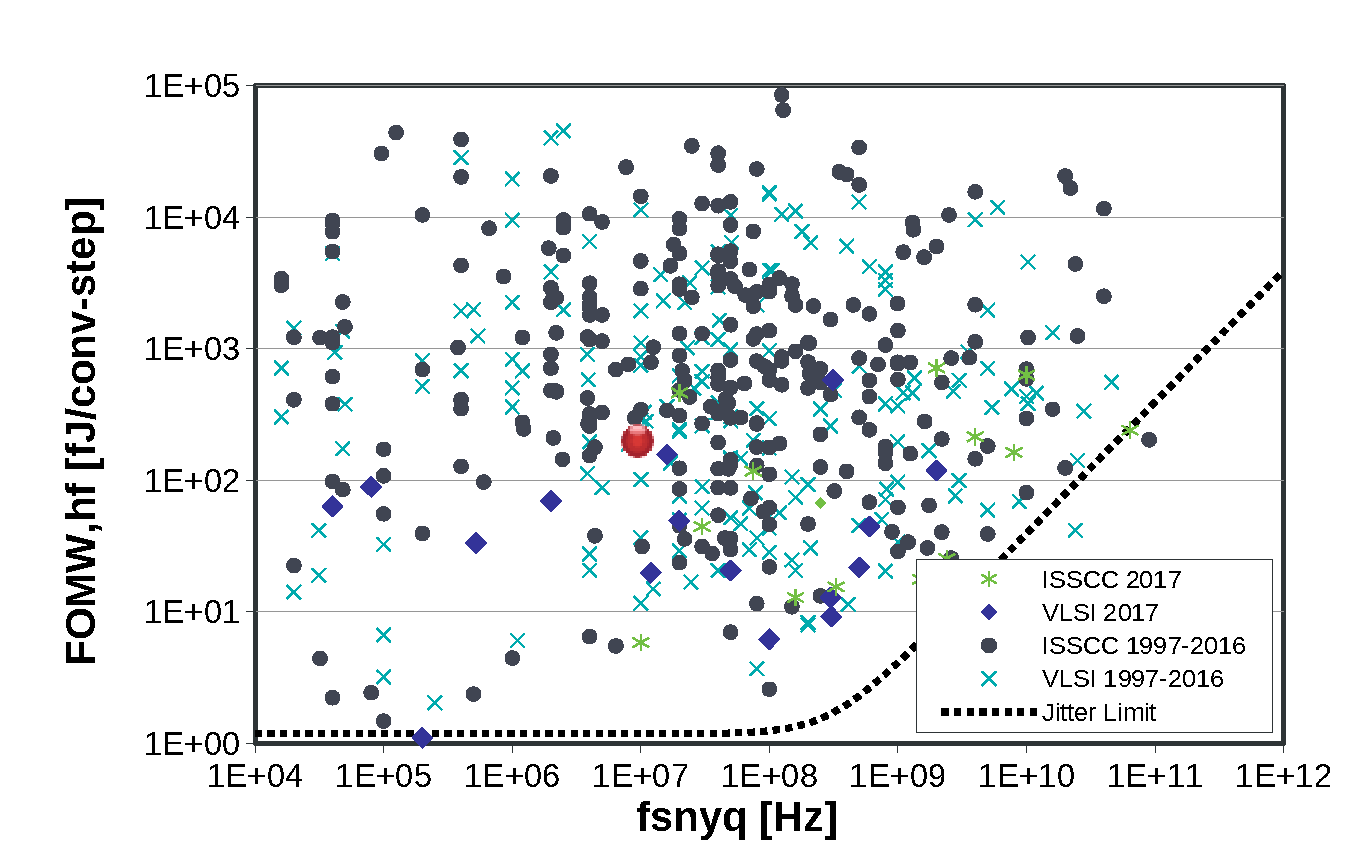
\includegraphics[width=\textwidth]{Abstract/Figs/WaldenFoM-a.pdf}
        a) Walden
    \end{minipage}
    \begin{minipage}[b]{0.49\linewidth}
        \centering
        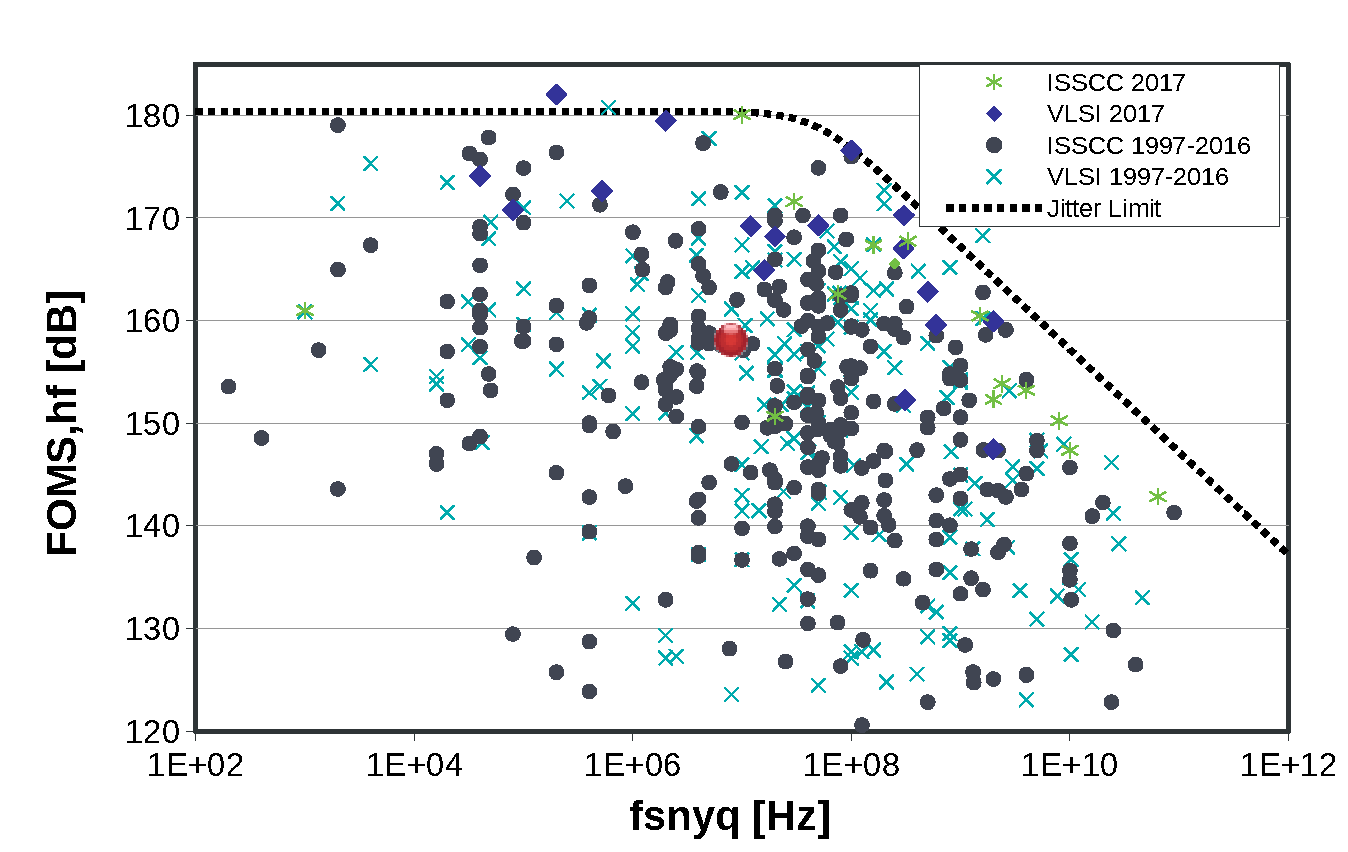
\includegraphics[width=\textwidth]{Abstract/Figs/SchreierFoM-a.pdf}
        b) Schreier
    \end{minipage}
    \caption[]{Comparaison du convertisseur (grand point rouge) a ceux publiées dans ISSCC et VLSI}
	\label{fig:fom-fr}
\end{center}

Afin d'améliorer cela, l'OTA pourrait être remplacé par une architecture moins gourmande, telle qu'une source de courant pilotée par un comparateur en temps continu, ou un ring amplifier. En plus de cela, une calibration numérique permettrait de relâcher la contrainte de timing et de toujours atteindre le nombre de bits effectifs.

L'environnement automobile est un défi pour la conception d'une électronique robuste. Exposés à des températures élevées, à des accélérations brusques et à de grandes variations de procédé de fabrication et de tension, beaucoup des innovations ont été explorées pour des capteurs intelligents adaptés à un marché piloté par la voiture autonome. À l'interface entre le capteur au sein de l'environnement sévère et l'unité de traitement, la tendance est de placer le convertisseur au plus près du capteur afin de bénéficier des avantages de l'électronique numérique en matière d'intégration, pour tirer parti d'algorithmes complexes, et pour économiser de l'énergie. Ainsi, l'invariabilité est donc le facteur clé de ces interfaces. Cependant, l’absence générale de progrès dans l’application de cette technique aux applications à haute température est évidente dans l'état de l'art.

L'objectif premier de ces travaux de recherche fut donc d'augmenter la stabilité du processus de conversion. Tout d'abord, cette stabilité vient du choix de l'architecture hybride proposée. En plus de cela, cette dernière admet une facilité de réutilisation avec une surface réduite à 0.12 $\rm mm^2$, et une consommation réduite à 8 mW. La gestion de puissance est alors moins contrainte.
% \end{small}
\end{mdframed}

\clearpage
\begin{mdframed}[linecolor=Prune,linewidth=1]
\vspace{-.25cm}
\paragraph*{Titre:} Analyse d’une nouvelle topologie fiable de convertisseur analogique-numérique pour \newline l'environnement automobile

\begin{small}
\vspace{-.25cm}
\paragraph*{Mot clés:} 

\vspace{-.5cm}
\begin{multicols}{2}
\paragraph*{Résumé:} 
La tendance du secteur automobile à développer des capteurs et actuateurs intelligents, l'électronique embarquée est l'art de faire cohabiter l'électronique analogique et l'électronique numérique. Placé au sein des actuateurs, ou au sein des boucles de régulation pour la sécurité et le confort des passagers, les convertisseurs analogique-numérique (CAN) sont les composants clés de ces systèmes intelligents. De plus, un CAN rapide, précis, et peu chère se révèle être un précieux allié pour les équipementiers. Pour diminuer les coûts, et augmenter la possible réutilisation de ce bloc, la surface de silicium occupée doit être considérablement réduite à moins de 0.5 $\rm mm^2$. Quant à la précision du convertisseur, 12-bits tous les 50 ns sont nécessaire pour la majorité des applications allant de -40\(\degree \)C à 175\(\degree \)C. A cela s'ajoute la volonté de réduire le taux de sur-échantillonnage à 5 coups d'horloge par échantillon.

Ce travail de recherche se focalise sur l'amélioration de l'efficacité énergétique sous les contraintes que l'environnement automobile représente. Notre principale contribution réside dans le développement par une approche top-down d'une nouvelle architecture à 3 étages de topologies différentes. Le premier étage, un $\Sigma\Delta$-Incrémental, est intrinsèquement linéaire. Le second étage est un algorithmique pour augmenter rapidement la résolution du convertisseur. Enfin, un SAR est utilisé pour accroître la résolution pour une faible augmentation de consommation de silicium et en courant.

Suite à l'analyse de 40 année d'état de l'art, la nouvelle architecture proposée fut validée par vérification des non-linéarité statique (DNL, INL) à différent niveaux de modélisation. Commençant par un modèle MATLAB sans les limitations analogique, le niveaux de modélisation se raffine petit à petit jusqu'à atteindre le niveau transistor du convertisseur. De ce faite, un modèle Verilog-A permet de déterminer les spécifications minimum des briques de base analogique: les comparateurs et les amplificateurs à transconductance. La sensibilité de ces derniers à la température fut analysé pour limiter les erreurs d'établissement commise sur les tensions analogiques. Une fois dessiné et les parasites extrait, ces modèles variant avec la température remplacent leur modèle Verilog-A respectif afin d'obtenir les performances finales. Parallèlement, deux architectures reconnus de comparateurs ont été évalué en température au sein d'une première puce de test. Dans laquel, deux méthodes ont été utilisés pour estimer l'offset des comparateurs, et un nouveau circuit asynchrone pour estimer le délai. Une seconde puce de test permet de vérifier la sensibilité du SAR à la température malgré un fonctionnement pseudo-asynchrone.

Pour les comparateurs, le nouveau circuit de mesure différentielle du retard montre une précision de 60 ps dans le pire des cas, pour le la plus petite surface sur puce connue en considérant la technologie utilisée. Comme la variation du retard est dépendant de la température, le choix d'un Strong-ARM ou une Double-Tail dépendra du bruit, de la puissance, de la tension d'alimentation, et spécification de kickback. Pour une tension d'alimentation standard, le comparateur de type Strong-ARM cible les systèmes à faible consommation avec une tolérance élevée pour le kickback différentiel. Au contraire, un comparateur Double-Tail accepte une plage de tension d'alimentation plus faible, et admet un faible kickback différentiel, mais présente un bruit plus important dû à l'intégrateur dans son premier étage. Testé de -40\(\degree \)C à 200\(\degree \)C, le dernier étage du CAN proposé n'a pas besoin d'être calibrée jusqu'à 180\(\degree \)C. Les résultats encourageants sur cette étage permettent la réutilisation de celui-ci pour calibrer les étages précédentes. Et pour le CAN, nous estimons une résolution possible de 11,2 bits en 5 cycles d'horloge par échantillon avec une extension à 13,3 bits en 6 cycles d'horloge. La surface estimée est de 0,12$mm^2$.

La puce de test pour le CAN n'étant pas encore fabriquée, une première étape sera sa caractérisation. Les résultats de cette session de mesure détermineront s'il est possible de pousser l'architecture à des fréquences plus élevés pour ensuite tirer parti du traitement numérique pour conserver les performances.
\end{multicols}
\end{small}
\end{mdframed}

\clearpage
\begin{mdframed}[linecolor=Prune,linewidth=1]
\vspace{-.25cm}
\paragraph*{Title:} A New ADC topology for reliable conversion in the automotive environment

\begin{small}
\vspace{-.25cm}
\paragraph*{Keywords:} 

\vspace{-.5cm}
\begin{multicols}{2}
\paragraph*{Abstract:} 
%-- paragraph de presentation
In the automotive industry, the trend being to develop smart sensors and actuators, the on-board electronic has been ever more an artful work to combine analog electronics and the digital one. While many monitoring and control systems play a crucial role as well for the safety as for the comfort of passengers, small components, like ADCs, are mandatory as a building block or as an essential functionality integrated into smart actuators. To that extent, a low-cost, fast and accurate analog to digital converter operating in those harsh conditions is a good ally for equipment manufacturers. To decrease the cost, the area is of primary concern. Considering re-use of the ADC as an IP-bloc, the area has been limited to less than half a square millimeter for an low-oversampling ratio of 5 to output a 12-bit code at a sample rate of 20 MSamples/s, over a wide temperature range from -40\(\degree \)C to 175\(\degree \)C.

%-- paragraph sur le but
This work focuses on the design of high-precision, high-speed and energy efficient ADC under the harsh environment the automotive one represents. Our main contribution relies on the development of an new hybrid topology proposal using 3 stages to cope with such constraints based on a top-down approach: A first counting stage inherently linear, an algorithmic stage allowing to increase rapidly the precision, and a SAR stage, ideal in terms of area and consumption, for a low number of bits.

%-- paragraph sur la method
Based on a 40 years literature review, a new topology proposal has been validated by checking its static metric of non-linearity (DNL, INL) at different level of modelisation. Starting by a MATLAB implementation without analog limitations, we refined step by step the model till we reach a transistor level of the ADC\@. Thence, Verilog-A model allows us to fix the minimum requirements of the key analog building blocks, to wit comparators and OTA\@. The latter has been analysed in order to limit the settling error sensitivity to the temperature. Laid-out, parasitic extracted simulation results of these considering PVT variations, they replace then previous high-level model to give final performances. Meanwhile, two well-known comparator architectures have been assessed as IP blocs inside a first test chip. To perform the offset extraction, both a conventional and a feedback loop have been inspected. To assess, the delay a new asynchronous circuit has been proposed. A second chip tests the sensitivity of the SAR to validate both the pseudo-asynchronous digital scheme, and a Double-Tail comparator in real operating conditions.

%-- paragraph sur les resultats
For comparators, the new differential measurement circuit of the delay demonstrate an accuracy of 60 ps in the worst case, over a large temperature range for the smallest chip area known with respect to the technology node size. The temperature variation of the delay being temperature dependent, the choice of a Strong-ARM or a Double-Tail hinge on the noise, power, supply voltage, and kickback specification. For standard power supply voltage, the Strong-ARM latch targets low-power systems application with a high tolerance for differential kickback. To the contrary, a Double-Tail latch allows lower power supply voltage range, with low-differential kickback. Otherwise, the Double-Tail exhibit a higher noise due to the integration in its first stage. Tested from -40$\degree$C to 200$\degree$C, the last stage of the proposed ADC topology does not need calibration up to 180$\degree$C. The encouraging results on this stage allows the re-use of the SAR to calibrate the previous stages. And considering the ADC, we estimate a possible resolution of 11.2-bits in 5 clock cycles per sample with an extension to 13.3-bits in 6 clock cycles with an estimated area of 0.12 $\rm mm^2$.

%-- paragraph sur les recommendations
The ADC test chip not being fabricated yet, a first step is the characterization of the ADC\@. From the results of the planned measurement session, the main goal is to push the architecture at higher sampling rates to then leverage the digital processing to enhance the sampling rate without changing the analog.
\end{multicols}
\end{small}
\end{mdframed}

%************************************
\vspace{3cm} % ALIGNER EN BAS DE PAGE
%************************************
\fontfamily{fvs}\fontseries{m}\selectfont
\begin{tabular}{p{14cm}r}
\multirow{3}{16cm}[+0mm]{{\color{Prune} Université Paris-Saclay\\
Espace Technologique / Immeuble Discovery\\
Route de l’Orme aux Merisiers RD 128 / 91190 Saint-Aubin, France}} & \multirow{3}{2.19cm}[+9mm]{
\includegraphics[height=2.19cm]{Figs/e.pdf}}\\
\end{tabular}